%%%%%%%%%%%%%%%%%%%%%%%%%%%%%%%%%%%%%%%%%
% The Legrand Orange Book
% LaTeX Template
% Version 2.0 (9/2/15)
%
% This template has been downloaded from:
% http://www.LaTeXTemplates.com
%
% Mathias Legrand (legrand.mathias@gmail.com) with modifications by:
% Vel (vel@latextemplates.com)
%
% License:
% CC BY-NC-SA 3.0 (http://creativecommons.org/licenses/by-nc-sa/3.0/)
%
% Compiling this template:
% This template uses biber for its bibliography and makeindex for its index.
% When you first open the template, compile it from the command line with the 
% commands below to make sure your LaTeX distribution is configured correctly:
%
% 1) pdflatex main
% 2) makeindex main.idx -s StyleInd.ist
% 3) biber main
% 4) pdflatex main x 2
%
% After this, when you wish to update the bibliography/index use the appropriate
% command above and make sure to compile with pdflatex several times 
% afterwards to propagate your changes to the document.
%
% This template also uses a number of packages which may need to be
% updated to the newest versions for the template to compile. It is strongly
% recommended you update your LaTeX distribution if you have any
% compilation errors.
%
% Important note:
% Chapter heading images should have a 2:1 width:height ratio,
% e.g. 920px width and 460px height.
%
%%%%%%%%%%%%%%%%%%%%%%%%%%%%%%%%%%%%%%%%%

%----------------------------------------------------------------------------------------
%	PACKAGES AND OTHER DOCUMENT CONFIGURATIONS
%----------------------------------------------------------------------------------------

\documentclass[12pt]{extbook} % Default font size and left-justified equations


%----------------------------------------------------------------------------------------
%	GRAYSCALE EM TODAS AS FIGURAS
% Habilita o modo impressão em tons de cinza, não todo logicmente
% Mas a maioria das coisas, as figuras não, isto é para mandar à editora em GRAY SCALE
%----------------------------------------------------------------------------------------
%\def\EnableGrayScale{1}

%----------------------------------------------------------------------------------------
%	GRAYSCALE EM TODAS AS FIGURAS
%----------------------------------------------------------------------------------------
\def \SourceRootPath{../../book}
%----------------------------------------------------------------------------------------

\usepackage{float}% para ter [H]
\usepackage{fancyvrb}

%----------------------------------------------------------------------------------------
%	DATOS DEL LIBRO
%----------------------------------------------------------------------------------------
\newcommand{\mytitle}[0]{M\'etodos num\'ericos}
\newcommand{\mysubtitle}[0]{Problemas n\~ao lineares e inversos}
\newcommand{\myauthor}[0]{Fernando Pujaico Rivera}
%----------------------------------------------------------------------------------------


%----------------------------------------------------------------------------------------
%	DATOS PATROCINIO
%----------------------------------------------------------------------------------------
\newcommand{\ImprimirLinkGitHub}[0]{https://localhost}%{https://trucomanx.github.io}
\newcommand{\ImprimirLinkHomePageLivro}[0]{\url{\ImprimirLinkGitHub/metodos.numericos}}
\newcommand{\ImprimirLinkVerificarLivro}[0]{\url{\ImprimirLinkGitHub/metodos.numericos/verificar.html}}
\newcommand{\ImprimirLinkCompraLivroImpresso}[0]{\url{\ImprimirLinkGitHub/metodos.numericos/comprar-impresso.html}}
\newcommand{\ImprimirLinkCompraLivroDigital}[0]{\url{\ImprimirLinkGitHub/metodos.numericos/comprar-digital.html}}
\newcommand{\ImprimirLinkMetodoPagoA}[0]{\url{https://apoia.se/metodosnumericos}}
%----------------------------------------------------------------------------------------
\newcommand{\ImprimirEmail}[0]{\href{mailto:fernando.pujaico.rivera@gmail.com}{fernando.pujaico.rivera@gmail.com}}

%----------------------------------------------------------------------------------------
%   DADOS ficha catalográfica
%----------------------------------------------------------------------------------------
\def \myauthorname{Fernando}
\def \myauthorlastname{Pujaico Rivera}
\def \myauthorborn{1982}
\def \imprimirlocal{Lavras}%cidade obrigatorio
\def \imprimiryear{2020}
\newcommand{\imprimirdata}[0]{\textcolor{red}{XXXXXXXXXXX} \imprimiryear}
\def \imprimirtipotrabalho{Inclui Bibliografia}
\def \imprimircuttersanborn{P979m} %% https://www.cuttersonline.com/app/generator/?q=Pujaico&ref=sanborn&add=
\newcommand{\imprimirpapersize}[0]{\textcolor{red}{XXXxXXXcm}} %21x30cm}
\def \imprimirCDD{515}   %% 515 Analysis https://www.oclc.org/content/dam/oclc/dewey/ddc23-summaries.pdf
                         %% 515.6 – Outros métodos analíticos %% Analysis %% https://books.google.com.br/books?id=BxeQiS_M2d0C
                         %% 515.6 – Outros métodos analíticos %% http://magisterandre.blogspot.com/2013/02/classificacao-decimal-de-dewey.html
                         %% http://www.isbn.bn.br/website/tabela-de-assuntos
\def \imprimirCDU{519.6} %% Matemática computacional %% https://www.ipleiria.pt/sdoc/wp-content/uploads/sites/10/2016/05/cdu-atualizada.pdf 
\newcommand{\imprimirisbn}[0]{\textcolor{red}{XXXXXXXXXXX}}
\def \imprimireditora{Edi\c{c}\~{a}o Independente}
\def \palavraschavea{M\'etodos num\'ericos}
\def \palavraschaveb{Problemas inversos}
\def \palavraschavec{C\'aculo num\'erico}
\def \palavraschavesInglesa{Numerical methods}
\def \palavraschavesInglesb{Inverse problems}
\def \palavraschavesInglesc{Numerical calculus}
%----------------------------------------------------------------------------------------

%\newcommand{\AnoLivro}[0]{2020}%% Ano da primeira edição, usado para ser trocado por: ATUALMENTE



%----------------------------------------------------------------------------------------
%	XCOLOR
%----------------------------------------------------------------------------------------
\usepackage[dvipsnames*,svgnames]{xcolor}

\definecolor{colorlowgray}{RGB}{240,240,240}
\definecolor{colorpartpagebackground}{RGB}{120,120,120} % lowgrayscale

\ifx\EnableGrayScale\undefined
    \definecolor{colorsystemdefault}{RGB}{16,81,15} % Define the color used for highlighting throughout the book
    \definecolor{colorsystemdefaultdkred}{RGB}{98,32,6} % Define the color used for highlighting throughout the book
    \definecolor{colorsystemdefaultdkblue}{RGB}{6,32,98} % Define the color used for highlighting throughout the book
    \definecolor{colormylink}{RGB}{16,120,15} % Define the 
    \definecolor{colorPatrocinio}{rgb}{0.98,0.88,0.82}
    \definecolor{colorAttention}{RGB}{255,249,128}
\else
    \definecolor{colorsystemdefault}{RGB}{0,0,0} % Define the color used for highlighting throughout the book
    \definecolor{colorsystemdefaultdkred}{RGB}{32,32,32} % Define the color used for highlighting throughout the book
    \definecolor{colorsystemdefaultdkblue}{RGB}{32,32,32} % Define the color used for highlighting throughout the book
    \definecolor{colormylink}{RGB}{64,64,64} % Define the 
    \definecolor{colorPatrocinio}{rgb}{0.98,0.98,0.98}
    \definecolor{colorAttention}{RGB}{255,255,255}
\fi



%----------------------------------------------------------------------------------------
%	COLOR
%----------------------------------------------------------------------------------------
\usepackage{color}


%----------------------------------------------------------------------------------------
% Força grayscale no livro
%----------------------------------------------------------------------------------------
%\ifx\EnableGrayScale\undefined
%    ~
%\else
%    \selectcolormodel{gray}
%\fi




%----------------------------------------------------------------------------------------
%----------------------------------------------------------------------------------------
%----------------------------------------------------------------------------------------


%----------------------------------------------------------------------------------------
%	VARIOUS REQUIRED PACKAGES AND CONFIGURATIONS
%----------------------------------------------------------------------------------------

\usepackage[top=2.5cm,bottom=2.5cm,left=2.5cm,right=2.5cm,headsep=10pt,a4paper]{geometry} % Page margins

\usepackage{graphicx} % Required for including pictures
\graphicspath{{pictures/}} % Specifies the directory where pictures are stored

\usepackage{lipsum} % Inserts dummy text

\usepackage[brazil]{babel}
%\usepackage[english]{babel} % English language/hyphenation

%----------------------------------------------------------------------------------------
%	Footnote
%----------------------------------------------------------------------------------------
\usepackage{scrextend} %multiple reference

%----------------------------------------------------------------------------------------
% Page counter
%----------------------------------------------------------------------------------------
\usepackage{lastpage}

%----------------------------------------------------------------------------------------
% GLOSSARIO
%----------------------------------------------------------------------------------------
\usepackage{nomencl}


%----------------------------------------------------------------------------------------
% Par diferentes modelos de caption.
%----------------------------------------------------------------------------------------
\usepackage{caption}
\usepackage{subcaption}
\usepackage{wrapfig}

%----------------------------------------------------------------------------------------
% Para \singlespacing 
%----------------------------------------------------------------------------------------
\usepackage{setspace}

%----------------------------------------------------------------------------------------
% Para 
% \begin{inparaenum}
% \item
% \end{inparaenum}
% parecido a timeze pero horizontal 
%----------------------------------------------------------------------------------------

\usepackage{paralist}

%----------------------------------------------------------------------------------------
% ROTATION FIGURE
%----------------------------------------------------------------------------------------
% For rotating figures, tables, etc.
%  including their captions
% \begin{sidewaysfigure}[ht]
% \end{sidewaysfigure}
\usepackage[figuresleft]{rotating}

%----------------------------------------------------------------------------------------
% MUSICAL NOTATION
%----------------------------------------------------------------------------------------
\usepackage[generate,ps2eps]{abc}%%sudo apt-get install abcm2ps
\usepackage[nointegrals]{wasysym}
\usepackage{harmony}


%----------------------------------------------------------------------------------------
% SIMILAR A ITEMIZE OU ENUMERATE
%----------------------------------------------------------------------------------------
\usepackage{tasks}

\settasks{
style=itemize, 
column-sep=5mm,
%label-format={\color{green!70!black}\large\bfseries},  
label-align=left, 
%label-offset={1mm}, 
%label-width={3mm}, 
%item-indent={1mm},
%item-format={\scshape\small}, 
%after-item-skip=1mm, 
%after-skip={10mm}
}


%----------------------------------------------------------------------------------------
% TABLE BREAKING
%----------------------------------------------------------------------------------------
\usepackage{longtable}

%----------------------------------------------------------------------------------------
% TABLE MULTIROW
%----------------------------------------------------------------------------------------

 \usepackage{multirow}

%----------------------------------------------------------------------------------------
% QR CODE
%----------------------------------------------------------------------------------------
%\usepackage{qrcode}

%----------------------------------------------------------------------------------------
% Grafico circulo satelites
%----------------------------------------------------------------------------------------
\usepackage{smartdiagram}
\usepackage{metalogo}
%\usepackage{dtklogos}



%----------------------------------------------------------------------------------------
%	BIBLIOGRAPHY AND INDEX
%----------------------------------------------------------------------------------------
 
\usepackage[ style=alphabetic,
             citestyle=alphabetic,
             sorting=none,
             sortcites=true,
             autopunct=true,
             babel=hyphen,
             hyperref=true,
             abbreviate=false,
             backref=true,
             backend=biber]{biblatex}
\addbibresource{bibliography/bibliography.bib} % BibTeX bibliography file
\defbibheading{bibempty}{}


\usepackage{calc} % For simpler calculation - used for spacing the index letter headings correctly
\usepackage{makeidx} % Required to make an index
\makeindex % Tells LaTeX to create the files required for indexing


 % paquetes usados con macros para la escrita
%%%%%%%%%%%%%%%%%%%%%%%%%%%%%%%%%%%%%%%%%
% The Legrand Orange Book
% Structural Definitions File
% Version 2.0 (9/2/15)
%
% Original author:
% Mathias Legrand (legrand.mathias@gmail.com) with modifications by:
% Vel (vel@latextemplates.com)
% 
% This file has been downloaded from:
% http://www.LaTeXTemplates.com
%
% License:
% CC BY-NC-SA 3.0 (http://creativecommons.org/licenses/by-nc-sa/3.0/)
%
%%%%%%%%%%%%%%%%%%%%%%%%%%%%%%%%%%%%%%%%%

%----------------------------------------------------------------------------------------
%	VARIOUS REQUIRED PACKAGES AND CONFIGURATIONS
%----------------------------------------------------------------------------------------

\usepackage[top=3cm,bottom=3cm,left=3cm,right=3cm,headsep=10pt,a4paper]{geometry} % Page margins

\usepackage{graphicx} % Required for including pictures
\graphicspath{{Pictures/}} % Specifies the directory where pictures are stored

\usepackage{lipsum} % Inserts dummy text

\usepackage{tikz} % Required for drawing custom shapes

\usepackage[english]{babel} % English language/hyphenation

\usepackage{enumitem} % Customize lists
\setlist{nolistsep} % Reduce spacing between bullet points and numbered lists

\usepackage{booktabs} % Required for nicer horizontal rules in tables

\usepackage{xcolor} % Required for specifying colors by name
%\definecolor{ocre}{RGB}{243,102,25} % Define the orange color used for highlighting throughout the book
\definecolor{ocre}{RGB}{16,81,15} % Define the orange color used for highlighting throughout the book

%----------------------------------------------------------------------------------------
%	FONTS
%----------------------------------------------------------------------------------------

\usepackage{avant} % Use the Avantgarde font for headings
%\usepackage{times} % Use the Times font for headings
\usepackage{mathptmx} % Use the Adobe Times Roman as the default text font together with math symbols from the Sym­bol, Chancery and Com­puter Modern fonts

\usepackage{microtype} % Slightly tweak font spacing for aesthetics
\usepackage[utf8]{inputenc} % Required for including letters with accents
\usepackage[T1]{fontenc} % Use 8-bit encoding that has 256 glyphs

%----------------------------------------------------------------------------------------
%	BIBLIOGRAPHY AND INDEX
%----------------------------------------------------------------------------------------

\usepackage[style=numeric,citestyle=numeric,sorting=nyt,sortcites=true,autopunct=true,babel=hyphen,hyperref=true,abbreviate=false,backref=true,backend=biber]{biblatex}
\addbibresource{bibliography.bib} % BibTeX bibliography file
\defbibheading{bibempty}{}

\usepackage{calc} % For simpler calculation - used for spacing the index letter headings correctly
\usepackage{makeidx} % Required to make an index
\makeindex % Tells LaTeX to create the files required for indexing

%----------------------------------------------------------------------------------------
%	MAIN TABLE OF CONTENTS
%----------------------------------------------------------------------------------------

\usepackage{titletoc} % Required for manipulating the table of contents

\contentsmargin{0cm} % Removes the default margin

% Part text styling
\titlecontents{part}[0cm]
{\addvspace{20pt}\centering\large\bfseries}
{}
{}
{}

% Chapter text styling
\titlecontents{chapter}[1.25cm] % Indentation
{\addvspace{12pt}\large\sffamily\bfseries} % Spacing and font options for chapters
{\color{ocre!60}\contentslabel[\Large\thecontentslabel]{1.25cm}\color{ocre}} % Chapter number
{\color{ocre}}  
{\color{ocre!60}\normalsize\;\titlerule*[.5pc]{.}\;\thecontentspage} % Page number

% Section text styling
\titlecontents{section}[1.25cm] % Indentation
{\addvspace{3pt}\sffamily\bfseries} % Spacing and font options for sections
{\contentslabel[\thecontentslabel]{1.25cm}} % Section number
{}
{\hfill\color{black}\thecontentspage} % Page number
[]

% Subsection text styling
\titlecontents{subsection}[1.25cm] % Indentation
{\addvspace{1pt}\sffamily\small} % Spacing and font options for subsections
{\contentslabel[\thecontentslabel]{1.25cm}} % Subsection number
{}
{\ \titlerule*[.5pc]{.}\;\thecontentspage} % Page number
[]

% List of figures
\titlecontents{figure}[0em]
{\addvspace{-5pt}\sffamily}
{\thecontentslabel\hspace*{1em}}
{}
{\ \titlerule*[.5pc]{.}\;\thecontentspage}
[]

% List of tables
\titlecontents{table}[0em]
{\addvspace{-5pt}\sffamily}
{\thecontentslabel\hspace*{1em}}
{}
{\ \titlerule*[.5pc]{.}\;\thecontentspage}
[]

%----------------------------------------------------------------------------------------
%	MINI TABLE OF CONTENTS IN PART HEADS
%----------------------------------------------------------------------------------------

% Chapter text styling
\titlecontents{lchapter}[0em] % Indenting
{\addvspace{15pt}\large\sffamily\bfseries} % Spacing and font options for chapters
{\color{ocre}\contentslabel[\Large\thecontentslabel]{1.25cm}\color{ocre}} % Chapter number
{}  
{\color{ocre}\normalsize\sffamily\bfseries\;\titlerule*[.5pc]{.}\;\thecontentspage} % Page number

% Section text styling
\titlecontents{lsection}[0em] % Indenting
{\sffamily\small} % Spacing and font options for sections
{\contentslabel[\thecontentslabel]{1.25cm}} % Section number
{}
{}

% Subsection text styling
\titlecontents{lsubsection}[.5em] % Indentation
{\normalfont\footnotesize\sffamily} % Font settings
{}
{}
{}

%----------------------------------------------------------------------------------------
%	PAGE HEADERS
%----------------------------------------------------------------------------------------

\usepackage{fancyhdr} % Required for header and footer configuration

\pagestyle{fancy}
\renewcommand{\chaptermark}[1]{\markboth{\sffamily\normalsize\bfseries\chaptername\ \thechapter.\ #1}{}} % Chapter text font settings
\renewcommand{\sectionmark}[1]{\markright{\sffamily\normalsize\thesection\hspace{5pt}#1}{}} % Section text font settings
\fancyhf{} \fancyhead[LE,RO]{\sffamily\normalsize\thepage} % Font setting for the page number in the header
\fancyhead[LO]{\rightmark} % Print the nearest section name on the left side of odd pages
\fancyhead[RE]{\leftmark} % Print the current chapter name on the right side of even pages
\renewcommand{\headrulewidth}{0.5pt} % Width of the rule under the header
\addtolength{\headheight}{2.5pt} % Increase the spacing around the header slightly
\renewcommand{\footrulewidth}{0pt} % Removes the rule in the footer
\fancypagestyle{plain}{\fancyhead{}\renewcommand{\headrulewidth}{0pt}} % Style for when a plain pagestyle is specified

% Removes the header from odd empty pages at the end of chapters
\makeatletter
\renewcommand{\cleardoublepage}{
\clearpage\ifodd\c@page\else
\hbox{}
\vspace*{\fill}
\thispagestyle{empty}
\newpage
\fi}

%----------------------------------------------------------------------------------------
%	THEOREM STYLES
%----------------------------------------------------------------------------------------

\usepackage{amsmath,amsfonts,amssymb,amsthm} % For math equations, theorems, symbols, etc

\newcommand{\intoo}[2]{\mathopen{]}#1\,;#2\mathclose{[}}
\newcommand{\ud}{\mathop{\mathrm{{}d}}\mathopen{}}
\newcommand{\intff}[2]{\mathopen{[}#1\,;#2\mathclose{]}}
\newtheorem{notation}{Notação}[chapter]

% Boxed/framed environments
\newtheoremstyle{ocrenumbox}% % Theorem style name
{0pt}% Space above
{0pt}% Space below
{\normalfont}% % Body font
{}% Indent amount
{\small\bf\sffamily\color{ocre}}% % Theorem head font
{\;}% Punctuation after theorem head
{0.25em}% Space after theorem head
{\small\sffamily\color{ocre}\thmname{#1}\nobreakspace\thmnumber{\@ifnotempty{#1}{}\@upn{#2}}% Theorem text (e.g. Theorem 2.1)
\thmnote{\nobreakspace\the\thm@notefont\sffamily\bfseries\color{black}---\nobreakspace#3.}} % Optional theorem note
\renewcommand{\qedsymbol}{$\blacksquare$}% Optional qed square

\newtheoremstyle{blacknumex}% Theorem style name
{5pt}% Space above
{5pt}% Space below
{\normalfont}% Body font
{} % Indent amount
{\small\bf\sffamily}% Theorem head font
{\;}% Punctuation after theorem head
{0.25em}% Space after theorem head
{\small\sffamily{\tiny\ensuremath{\blacksquare}}\nobreakspace\thmname{#1}\nobreakspace\thmnumber{\@ifnotempty{#1}{}\@upn{#2}}% Theorem text (e.g. Theorem 2.1)
\thmnote{\nobreakspace\the\thm@notefont\sffamily\bfseries---\nobreakspace#3.}}% Optional theorem note

\newtheoremstyle{blacknumbox} % Theorem style name
{0pt}% Space above
{0pt}% Space below
{\normalfont}% Body font
{}% Indent amount
{\small\bf\sffamily}% Theorem head font
{\;}% Punctuation after theorem head
{0.25em}% Space after theorem head
{\small\sffamily\thmname{#1}\nobreakspace\thmnumber{\@ifnotempty{#1}{}\@upn{#2}}% Theorem text (e.g. Theorem 2.1)
\thmnote{\nobreakspace\the\thm@notefont\sffamily\bfseries---\nobreakspace#3.}}% Optional theorem note

% Non-boxed/non-framed environments
\newtheoremstyle{ocrenum}% % Theorem style name
{5pt}% Space above
{5pt}% Space below
{\normalfont}% % Body font
{}% Indent amount
{\small\bf\sffamily\color{ocre}}% % Theorem head font
{\;}% Punctuation after theorem head
{0.25em}% Space after theorem head
{\small\sffamily\color{ocre}\thmname{#1}\nobreakspace\thmnumber{\@ifnotempty{#1}{}\@upn{#2}}% Theorem text (e.g. Theorem 2.1)
\thmnote{\nobreakspace\the\thm@notefont\sffamily\bfseries\color{black}---\nobreakspace#3.}} % Optional theorem note
\renewcommand{\qedsymbol}{$\blacksquare$}% Optional qed square
\makeatother

% Defines the theorem text style for each type of theorem to one of the three styles above
\newcounter{dummy} 
\numberwithin{dummy}{section}
\theoremstyle{ocrenumbox}
\newtheorem{theoremeT}[dummy]{Teorema}
\newtheorem{problemT}{Problema}[chapter]
\newtheorem{exerciseT}{Exercise}[chapter]
\theoremstyle{blacknumex}
\newtheorem{exampleT}{Example}[chapter]
\theoremstyle{blacknumbox}
\newtheorem{vocabulary}{Vocabulary}[chapter]
\newtheorem{definitionT}{Definição}[section]
\newtheorem{corollaryT}[dummy]{Corolário}
\newtheorem{myproofT}{Prova} [chapter]
\theoremstyle{ocrenum}
\newtheorem{propositionT}[dummy]{Proposição}

%----------------------------------------------------------------------------------------
%	DEFINITION OF COLORED BOXES
%----------------------------------------------------------------------------------------

\RequirePackage[framemethod=default]{mdframed} % Required for creating the theorem, definition, exercise and corollary boxes

% Theorem box
\newmdenv[skipabove=7pt,
skipbelow=7pt,
backgroundcolor=black!5,
linecolor=ocre,
innerleftmargin=5pt,
innerrightmargin=5pt,
innertopmargin=5pt,
leftmargin=0cm,
rightmargin=0cm,
innerbottommargin=5pt]{tBox}

% Proposition box
\newmdenv[skipabove=7pt,
skipbelow=7pt,
backgroundcolor=blue!5,
linecolor=ocre,
innerleftmargin=5pt,
innerrightmargin=5pt,
innertopmargin=5pt,
leftmargin=0cm,
rightmargin=0cm,
innerbottommargin=5pt]{ppBox}

% Exercise box	  
\newmdenv[skipabove=7pt,
skipbelow=7pt,
rightline=false,
leftline=true,
topline=false,
bottomline=false,
backgroundcolor=ocre!10,
linecolor=ocre,
innerleftmargin=5pt,
innerrightmargin=5pt,
innertopmargin=5pt,
innerbottommargin=5pt,
leftmargin=0cm,
rightmargin=0cm,
linewidth=4pt]{eBox}	


% Problem box	  
\newmdenv[skipabove=7pt,
skipbelow=7pt,
rightline=false,
leftline=true,
topline=false,
bottomline=false,
backgroundcolor=ocre!10,
linecolor=ocre,
innerleftmargin=5pt,
innerrightmargin=5pt,
innertopmargin=5pt,
innerbottommargin=5pt,
leftmargin=0cm,
rightmargin=0cm,
linewidth=4pt]{pBox}	

% Definition box
\newmdenv[skipabove=7pt,
skipbelow=7pt,
rightline=false,
leftline=true,
topline=false,
bottomline=false,
linecolor=ocre,
innerleftmargin=5pt,
innerrightmargin=5pt,
innertopmargin=0pt,
leftmargin=0cm,
rightmargin=0cm,
linewidth=4pt,
innerbottommargin=0pt]{dBox}	

% Corollary box
\newmdenv[skipabove=7pt,
skipbelow=7pt,
rightline=false,
leftline=true,
topline=false,
bottomline=false,
linecolor=gray,
backgroundcolor=black!5,
innerleftmargin=5pt,
innerrightmargin=5pt,
innertopmargin=5pt,
leftmargin=0cm,
rightmargin=0cm,
linewidth=4pt,
innerbottommargin=5pt]{cBox}

% Creates an environment for each type of theorem and assigns it a theorem text style from the "Theorem Styles" section above and a colored box from above
\newenvironment{theorem}{\begin{tBox}\begin{theoremeT}}{\end{theoremeT}\end{tBox}}
\newenvironment{proposition}{\begin{ppBox}\begin{propositionT}}{\end{propositionT}\end{ppBox}}
\newenvironment{exercise}{\begin{eBox}\begin{exerciseT}}{\hfill{\color{ocre}\tiny\ensuremath{\blacksquare}}\end{exerciseT}\end{eBox}}			
\newenvironment{problem}{\begin{pBox}\begin{problemT}}{\hfill{\color{ocre}\tiny\ensuremath{\blacksquare}}\end{problemT}\end{pBox}}				  
\newenvironment{definition}{\begin{dBox}\begin{definitionT}}{\end{definitionT}\end{dBox}}	
\newenvironment{example}{\begin{exampleT}}{\hfill{\tiny\ensuremath{\blacksquare}}\end{exampleT}}		
\newenvironment{corollary}{\begin{cBox}\begin{corollaryT}}{\end{corollaryT}\end{cBox}}	

%----------------------------------------------------------------------------------------
%	REMARK ENVIRONMENT
%----------------------------------------------------------------------------------------

\newenvironment{remark}{\par\vspace{10pt}\small % Vertical white space above the remark and smaller font size
\begin{list}{}{
\leftmargin=35pt % Indentation on the left
\rightmargin=25pt}\item\ignorespaces % Indentation on the right
\makebox[-2.5pt]{\begin{tikzpicture}[overlay]
\node[draw=ocre!60,line width=1pt,circle,fill=ocre!25,font=\sffamily\bfseries,inner sep=2pt,outer sep=0pt] at (-15pt,0pt){\textcolor{ocre}{R}};\end{tikzpicture}} % Orange R in a circle
\advance\baselineskip -1pt}{\end{list}\vskip5pt} % Tighter line spacing and white space after remark

%----------------------------------------------------------------------------------------
%	SECTION NUMBERING IN THE MARGIN
%----------------------------------------------------------------------------------------

\makeatletter
\renewcommand{\@seccntformat}[1]{\llap{\textcolor{ocre}{\csname the#1\endcsname}\hspace{1em}}}                    
\renewcommand{\section}{\@startsection{section}{1}{\z@}
{-4ex \@plus -1ex \@minus -.4ex}
{1ex \@plus.2ex }
{\normalfont\large\sffamily\bfseries}}
\renewcommand{\subsection}{\@startsection {subsection}{2}{\z@}
{-3ex \@plus -0.1ex \@minus -.4ex}
{0.5ex \@plus.2ex }
{\normalfont\sffamily\bfseries}}
\renewcommand{\subsubsection}{\@startsection {subsubsection}{3}{\z@}
{-2ex \@plus -0.1ex \@minus -.2ex}
{.2ex \@plus.2ex }
{\normalfont\small\sffamily\bfseries}}                        
\renewcommand\paragraph{\@startsection{paragraph}{4}{\z@}
{-2ex \@plus-.2ex \@minus .2ex}
{.1ex}
{\normalfont\small\sffamily\bfseries}}

%----------------------------------------------------------------------------------------
%	PART HEADINGS
%----------------------------------------------------------------------------------------

% numbered part in the table of contents
\newcommand{\@mypartnumtocformat}[2]{%
\setlength\fboxsep{0pt}%
\noindent\colorbox{ocre!20}{\strut\parbox[c][.7cm]{\ecart}{\color{ocre!70}\Large\sffamily\bfseries\centering#1}}\hskip\esp\colorbox{ocre!40}{\strut\parbox[c][.7cm]{\linewidth-\ecart-\esp}{\Large\sffamily\centering#2}}}%
%%%%%%%%%%%%%%%%%%%%%%%%%%%%%%%%%%
% unnumbered part in the table of contents
\newcommand{\@myparttocformat}[1]{%
\setlength\fboxsep{0pt}%
\noindent\colorbox{ocre!40}{\strut\parbox[c][.7cm]{\linewidth}{\Large\sffamily\centering#1}}}%
%%%%%%%%%%%%%%%%%%%%%%%%%%%%%%%%%%
\newlength\esp
\setlength\esp{4pt}
\newlength\ecart
\setlength\ecart{1.2cm-\esp}
\newcommand{\thepartimage}{}%
\newcommand{\partimage}[1]{\renewcommand{\thepartimage}{#1}}%
\def\@part[#1]#2{%
\ifnum \c@secnumdepth >-2\relax%
\refstepcounter{part}%
\addcontentsline{toc}{part}{\texorpdfstring{\protect\@mypartnumtocformat{\thepart}{#1}}{\partname~\thepart\ ---\ #1}}
\else%
\addcontentsline{toc}{part}{\texorpdfstring{\protect\@myparttocformat{#1}}{#1}}%
\fi%
\startcontents%
\markboth{}{}%
{\thispagestyle{empty}%
\begin{tikzpicture}[remember picture,overlay]%
\node at (current page.north west){\begin{tikzpicture}[remember picture,overlay]%	
\fill[ocre!20](0cm,0cm) rectangle (\paperwidth,-\paperheight);
\node[anchor=north] at (4cm,-3.25cm){\color{ocre!40}\fontsize{220}{100}\sffamily\bfseries\@Roman\c@part}; 
\node[anchor=south east] at (\paperwidth-1cm,-\paperheight+1cm){\parbox[t][][t]{8.5cm}{
\printcontents{l}{0}{\setcounter{tocdepth}{1}}%
}};
\node[anchor=north east] at (\paperwidth-1.5cm,-3.25cm){\parbox[t][][t]{15cm}{\strut\raggedleft\color{white}\fontsize{30}{30}\sffamily\bfseries#2}};
\end{tikzpicture}};
\end{tikzpicture}}%
\@endpart}
\def\@spart#1{%
\startcontents%
\phantomsection
{\thispagestyle{empty}%
\begin{tikzpicture}[remember picture,overlay]%
\node at (current page.north west){\begin{tikzpicture}[remember picture,overlay]%	
\fill[ocre!20](0cm,0cm) rectangle (\paperwidth,-\paperheight);
\node[anchor=north east] at (\paperwidth-1.5cm,-3.25cm){\parbox[t][][t]{15cm}{\strut\raggedleft\color{white}\fontsize{30}{30}\sffamily\bfseries#1}};
\end{tikzpicture}};
\end{tikzpicture}}
\addcontentsline{toc}{part}{\texorpdfstring{%
\setlength\fboxsep{0pt}%
\noindent\protect\colorbox{ocre!40}{\strut\protect\parbox[c][.7cm]{\linewidth}{\Large\sffamily\protect\centering #1\quad\mbox{}}}}{#1}}%
\@endpart}
\def\@endpart{\vfil\newpage
\if@twoside
\if@openright
\null
\thispagestyle{empty}%
\newpage
\fi
\fi
\if@tempswa
\twocolumn
\fi}

%----------------------------------------------------------------------------------------
%	CHAPTER HEADINGS
%----------------------------------------------------------------------------------------

\newcommand{\thechapterimage}{}%
\newcommand{\chapterimage}[1]{\renewcommand{\thechapterimage}{#1}}%
\def\@makechapterhead#1{%
{\parindent \z@ \raggedright \normalfont
\ifnum \c@secnumdepth >\m@ne
\if@mainmatter
\begin{tikzpicture}[remember picture,overlay]
\node at (current page.north west)
{\begin{tikzpicture}[remember picture,overlay]
\node[anchor=north west,inner sep=0pt] at (0,0) {\includegraphics[width=\paperwidth]{\thechapterimage}};
\draw[anchor=west] (\Gm@lmargin,-9cm) node [line width=2pt,rounded corners=15pt,draw=ocre,fill=white,fill opacity=0.5,inner sep=15pt]{\strut\makebox[22cm]{}};
\draw[anchor=west] (\Gm@lmargin+.3cm,-9cm) node {\huge\sffamily\bfseries\color{black}\thechapter. #1\strut};
\end{tikzpicture}};
\end{tikzpicture}
\else
\begin{tikzpicture}[remember picture,overlay]
\node at (current page.north west)
{\begin{tikzpicture}[remember picture,overlay]
\node[anchor=north west,inner sep=0pt] at (0,0) {\includegraphics[width=\paperwidth]{\thechapterimage}};
\draw[anchor=west] (\Gm@lmargin,-9cm) node [line width=2pt,rounded corners=15pt,draw=ocre,fill=white,fill opacity=0.5,inner sep=15pt]{\strut\makebox[22cm]{}};
\draw[anchor=west] (\Gm@lmargin+.3cm,-9cm) node {\huge\sffamily\bfseries\color{black}#1\strut};
\end{tikzpicture}};
\end{tikzpicture}
\fi\fi\par\vspace*{270\p@}}}

%-------------------------------------------

\def\@makeschapterhead#1{%
\begin{tikzpicture}[remember picture,overlay]
\node at (current page.north west)
{\begin{tikzpicture}[remember picture,overlay]
\node[anchor=north west,inner sep=0pt] at (0,0) {\includegraphics[width=\paperwidth]{\thechapterimage}};
\draw[anchor=west] (\Gm@lmargin,-9cm) node [line width=2pt,rounded corners=15pt,draw=ocre,fill=white,fill opacity=0.5,inner sep=15pt]{\strut\makebox[22cm]{}};
\draw[anchor=west] (\Gm@lmargin+.3cm,-9cm) node {\huge\sffamily\bfseries\color{black}#1\strut};
\end{tikzpicture}};
\end{tikzpicture}
\par\vspace*{270\p@}}
\makeatother

%----------------------------------------------------------------------------------------
%	HYPERLINKS IN THE DOCUMENTS
%----------------------------------------------------------------------------------------

\usepackage{hyperref}
\hypersetup{hidelinks,backref=true,pagebackref=true,hyperindex=true,colorlinks=false,breaklinks=true,urlcolor= ocre,bookmarks=true,bookmarksopen=false,pdftitle={Title},pdfauthor={Author}}
\usepackage{bookmark}
\bookmarksetup{
open,
numbered,
addtohook={%
\ifnum\bookmarkget{level}=0 % chapter
\bookmarksetup{bold}%
\fi
\ifnum\bookmarkget{level}=-1 % part
\bookmarksetup{color=ocre,bold}%
\fi
}
}
 % el estilo visual do livro

%----------------------------------------------------------------------------------------
%  footnote font size
%----------------------------------------------------------------------------------------
\renewcommand{\footnotesize}{\small}

%----------------------------------------------------------------------------------------
%	Horizontal separator line
%   \HRule{2pt}
%----------------------------------------------------------------------------------------
\newcommand{\HRule}[1]{\rule{\linewidth}{#1}} % creo el comando  \HRule regla horizontal



%----------------------------------------------------------------------------------------
%	Horizontal separator line
%   \PRLsep{Text}
%----------------------------------------------------------------------------------------
\newlength{\PRLlen}
\newcommand*\PRLsep[1]{\settowidth{\PRLlen}{#1}\advance\PRLlen by -\textwidth\divide\PRLlen by -2\noindent\makebox[\the\PRLlen]{\resizebox{\the\PRLlen}{1pt}{$\blacktriangleleft$}}\raisebox{-.5ex}{\textbf{#1}}\makebox[\the\PRLlen]{\resizebox{\the\PRLlen}{1pt}{$\blacktriangleright$}}\bigskip}


%----------------------------------------------------------------------------------------
%----------------------------------------------------------------------------------------
%----------------------------------------------------------------------------------------
%----------------------------------------------------------------------------------------
% BOX - TCOLORBOX
%----------------------------------------------------------------------------------------
\usepackage[most,many]{tcolorbox}
\usetikzlibrary{decorations.pathmorphing}
\tcbuselibrary{skins}
%----------------------------------------------------------------------------------------
% ATTENTION MESSAGE BOX
%----------------------------------------------------------------------------------------
% \begin{tcbattention}
%   text
% \end{tcbattention}
%%\newtcolorbox{tcbattention}
%%{
%%  breakable,
%%  enhanced,
%%  arc      =1mm,
%%  colback  =colorsystemdefaultdkred!5,
%%  colframe =colorsystemdefaultdkred,
%%  leftrule =14mm,%
%%  drop fuzzy shadow=black,
%%  overlay  ={\node[anchor=north west,outer sep=4pt] at (frame.north west) {
\includegraphics[width=8mm]{attention1.eps}}; }
%%}

\newtcolorbox{tcbattention}[1][]{enhanced,
  before skip=2mm,after skip=3mm,
  boxrule=0.4pt,left=5mm,right=2mm,top=1mm,bottom=1mm,
  colback=yellow!50,
  colframe=yellow!20!black,
  sharp corners,rounded corners=southeast,arc is angular,arc=3mm,
  underlay={%
    \path[fill=colorsystemdefault!20!black] ([yshift=3mm]interior.south east)--++(-0.4,-0.1)--++(0.1,-0.2);
    \path[draw=colorsystemdefault,shorten <=-0.05mm,shorten >=-0.05mm] ([yshift=3mm]interior.south east)--++(-0.4,-0.1)--++(0.1,-0.2);
    \path[fill=yellow!50!black,draw=none] (interior.south west) rectangle node[white]{\Huge\bfseries !} ([xshift=4mm]interior.north west);
    },
  drop fuzzy shadow,#1}
%----------------------------------------------------------------------------------------
% INFORMATION MESSAGE BOX
%----------------------------------------------------------------------------------------
\newtcolorbox{tcbinformation}%[1]
{
  %title=#1,
  %fonttitle=\bfseries,
  breakable,
  enhanced,
  arc      =1mm,
  colback  =colorsystemdefault!5,
  colframe =colorsystemdefault,
  leftrule =14mm,%
  drop fuzzy shadow=black,
  overlay  ={\node[anchor=north west,outer sep=4pt] at (frame.north west) {
\includegraphics[width=8mm]{information1.eps}}; }
}



%----------------------------------------------------------------------------------------
% ELABORACION MESSAGE BOX
%----------------------------------------------------------------------------------------
% \begin{elaboracion}[title=título, width= 0.80\linewidth]
%   texto
% \end{elaboracion}
\newtcolorbox{elaboracion}[1][]{
    tile,
    colback=fboxbackcolor!5,
    coltitle=white,
    colbacktitle=fboxfrontcolor,%fboxfrontcolor!10,
    center title,
    toprule=1.25mm,
    bottomrule=1.25mm,
    extras unbroken and first={borderline north={0.5mm}{0.5mm}{fboxfrontcolor,decoration={zigzag,amplitude=0.5mm},decorate}},
    extras unbroken and last={borderline south={0.5mm}{0.5mm}{fboxfrontcolor,decoration={zigzag,amplitude=0.5mm},decorate}},
    #1
}

%----------------------------------------------------------------------------------------
% CITANDO MESSAGE BOX
%----------------------------------------------------------------------------------------
% \begin{citando}
%   texto
% \end{citando}
\newtcolorbox{citando}
{
  breakable,
  enhanced,
  colback  = colorlowgray,
  colframe = colorlowgray,
  arc      = 3mm,
  left skip= 0.10 \linewidth,
  width    = 0.90 \linewidth
}


%----------------------------------------------------------------------------------------
% CARACTERISTICAS MESSAGE BOX
%----------------------------------------------------------------------------------------
\usepackage{pifont}
\newcommand{\CheckedItem}{\rlap{$\square$}{\large\hspace{0pt}\ding{51}}}
\newcommand{\NoCheckedItem}{\rlap{$\square$}{\large\hspace{13pt}}}

%----------------------------------------------------------------------------------------
% \caracterpasso{\CheckedItem}{\CheckedItem}{\NoCheckedItem}{\CheckedItem}{4}

\colorlet{fboxbackcolorpasso}{colorsystemdefault!66!blue}
\colorlet{fboxfrontcolorpasso}{colorsystemdefault!66!blue}

\newtcolorbox{tcbcaracteristicapasso}[1][]{
    tile,
    colback=fboxbackcolorpasso!5,
    coltitle=white,
    colbacktitle=fboxfrontcolorpasso,%fboxfrontcolor!10,
    center title,
    toprule=1.25mm,
    bottomrule=1.25mm,
    extras unbroken and first={borderline north={0.5mm}{0.5mm}{fboxfrontcolorpasso,decoration={zigzag,amplitude=0.5mm},decorate}},
    extras unbroken and last={borderline south={0.5mm}{0.5mm}{fboxfrontcolorpasso,decoration={zigzag,amplitude=0.5mm},decorate}},
    #1
}



\newcommand{\caracterpasso}[5]{
\begin{wrapfigure}{l}{0.5\textwidth} 
\begin{tcbcaracteristicapasso}[title=Caraterísticas, width= \linewidth]
 \begin{itemize}
\item[#1] \hyperref[def:PassoCiclico]{\textbf{Passo cíclico}}.
\item[#2] \hyperref[def:PassoSimetrico]{\textbf{Passo simétrico}}.
\item[#3] \hyperref[def:PassoAContratempo]{\textbf{Passo a contratempo}}.
\item[#4] \hyperref[def:PassoDeDeslocamento]{\textbf{Passo de deslocamento}}.
\item     \hyperref[def:DuracaoDoPasso]{\textbf{Duração}}: #5 tempos.
\end{itemize}
\end{tcbcaracteristicapasso}
\end{wrapfigure}
}


%----------------------------------------------------------------------------------------
% \caracterpostura{\CheckedItem}{{\NoCheckedItem}

\colorlet{fboxbackcolorpostura}{colorsystemdefault!66!red}
\colorlet{fboxfrontcolorpostura}{colorsystemdefault!66!red}

\newtcolorbox{tcbcaracteristicapostura}[1][]{
    tile,
    colback=fboxbackcolorpostura!5,
    coltitle=white,
    colbacktitle=fboxfrontcolorpostura,%fboxfrontcolor!10,
    center title,
    toprule=1.25mm,
    bottomrule=1.25mm,
    extras unbroken and first={borderline north={0.5mm}{0.5mm}{fboxfrontcolorpostura,decoration={zigzag,amplitude=0.5mm},decorate}},
    extras unbroken and last={borderline south={0.5mm}{0.5mm}{fboxfrontcolorpostura,decoration={zigzag,amplitude=0.5mm},decorate}},
    #1
}


\newcommand{\caracterpostura}[2]{
\begin{wrapfigure}{l}{0.5\textwidth} 
\begin{tcbcaracteristicapostura}[title=Caraterísticas, width= \linewidth]
 \begin{itemize}
\item[#1] \hyperref[def:PosturaFinaliza]{\textbf{Postura de finalização}}.
\item[#2] \hyperref[def:PosturaTransicao]{\textbf{Postura de transição}}.
\end{itemize}
\end{tcbcaracteristicapostura}
\end{wrapfigure}
}





%----------------------------------------------------------------------------------------
% TABULARTCB
%----------------------------------------------------------------------------------------
% \caracterelement{Algum texto 1}{Algum texto 2}

\colorlet{fboxbackcolorelement}{colorsystemdefault}
\colorlet{fboxfrontcolorelement}{colorsystemdefault}

\newtcolorbox{tcbcaracterelement}[1][]{
    tile,
    colback=fboxbackcolorelement!5,
    coltitle=white,
    colbacktitle=fboxfrontcolorelement,%fboxfrontcolor!10,
    center title,
    toprule=1.25mm,
    bottomrule=1.25mm,
    extras unbroken and first={borderline north={0.5mm}{0.5mm}{fboxfrontcolorelement,decoration={zigzag,amplitude=0.5mm},decorate}},
    extras unbroken and last={borderline south={0.5mm}{0.5mm}{fboxfrontcolorelement,decoration={zigzag,amplitude=0.5mm},decorate}},
    #1
}



\newcommand{\caracterelement}[2]{
\begin{wrapfigure}{l}{0.6\textwidth} 
\begin{tcbcaracterelement}[title=Caraterísticas, width= \linewidth]
\begin{tabular}{rp{0.6\textwidth}}
\textbf{Consciência:} & #1 \\
\textbf{Pergunta:}    & #2
\end{tabular} 
\end{tcbcaracterelement}
\end{wrapfigure}
}




%----------------------------------------------------------------------------------------
% FRASES E DITADOS
%----------------------------------------------------------------------------------------
% \begin{FraseFernandoPR}{Frase}
% meu texto
% \end{FraseFernandoPR}


\newtcolorbox[auto counter]{FraseFernandoPR}{
freelance,
colback=white,
frame code={},
interior titled code={
  \fill[rounded corners=8pt,colorsystemdefault!30]
    (title.south west) --
    (title.south) -- 
    ([yshift=15pt]title.south) --
    ([yshift=15pt,xshift=4cm]title.south) --
    ([xshift=4cm]title.south) --
    (title.south east) {[sharp corners] --
    ([yshift=-6pt]title.south east) -- 
    ([yshift=-6pt]title.south west) } -- cycle;
  \draw[rounded corners=8pt,colorsystemdefault,line width=1pt]
    (title.west|-frame.south west) --
    (title.south west) --
    (title.south) -- 
    ([yshift=15pt]title.south) --
    ([yshift=15pt,xshift=4cm]title.south) --
    ([xshift=4cm]title.south) --
    (title.south east) --
    (title.east|-frame.south east) --
    cycle;
  \node at ([xshift=2cm,yshift=4pt,anchor=south]title.south) 
    { \bfseries  Frase~\thetcbcounter};  
  },
title={\mbox{}},
top=12pt,
%fontupper=\sffamily\Large,
oversize=0.0cm,
after upper={\\{  \mbox{} \hfill Fernando P.R.}\index{Frases e Ditados}},
before={\vskip 24pt\par\noindent},
after={\par\vskip 12pt}
}


%%%%%%%%%%%%%%%%%%%%%%%%%%%%%%%%%%%%%%%%%%%%%%%%%%%%%%%%%%%%%%%%%%%%%%%%%%%%%%%%
%%%%%%%%%%%%%%%%%%%%%%%%%%%%%%%%%%%%%%%%%%%%%%%%%%%%%%%%%%%%%%%%%%%%%%%%%%%%%%%%
%%%%%%%%%%%%%%%%%%%%%%%%%%%%%%%%%%%%%%%%%%%%%%%%%%%%%%%%%%%%%%%%%%%%%%%%%%%%%%%%
%%%%%%%%%%%%%%%%%%%%%%%%%%%%%%%%%%%%%%%%%%%%%%%%%%%%%%%%%%%%%%%%%%%%%%%%%%%%%%%%
%% UN SOLO USO
%%%%%%%%%%%%%%%%%%%%%%%%%%%%%%%%%%%%%%%%%%%%%%%%%%%%%%%%%%%%%%%%%%%%%%%%%%%%%%%%


%----------------------------------------------------------------------------------------
% CATALOGRAFICA MESSAGE BOX
%----------------------------------------------------------------------------------------
% \begin{catalografica}
%   texto
% \end{catalografica}
\newtcolorbox{catalografica}
{
  breakable,
  enhanced,
  colback  = colorlowgray,
  colframe = colorlowgray
}


%----------------------------------------------------------------------------------------
% PATROCINIO MESSAGE BOX
%----------------------------------------------------------------------------------------
% \begin{patrocinio}
%   texto
% \end{patrocinio}
\newtcolorbox{patrocinio}
{
  breakable,
  enhanced,
  colback  = colorlowred,
  colframe = colorlowred
}


 % las macros compuestas usadas para la escrita

%-----------------------------------------------------------------------------------------
% evitar linhas órfãs e viúvas
%\clubpenalty=100000 
%\widowpenalty=100000 
%-----------------------------------------------------------------------------------------

\hyphenation{sam-ba}
\hyphenation{Har-wood}
\hyphenation{mo-vi-men-tar}
\hyphenation{mo-vi-men-tar-nos}

%----------------------------------------------------------------------------------------
% Para a criação do Glossário
%----------------------------------------------------------------------------------------
\makenomenclature

%%%%%%%%%%%%%%%%%%%%%%%%%%%%%%%%%%%%%%%%%%%%%%%%%%%%%%%%%%%%%%%%%%%%%%%%%%%%%%%%%%
\renewcommand*{\bibfont}{\footnotesize}
%%%%%%%%%%%%%%%%%%%%%%%%%%%%%%%%%%%%%%%%%%%%%%%%%%%%%%%%%%%%%%%%%%%%%%%%%%%%%%%%%%
%%%%%%%%%%%%%%%%%%%%%%%%%%%%%%%%%%%%%%%%%%%%%%%%%%%%%%%%%%%%%%%%%%%%%%%%%%%%%%%%%%


%----------------------------------------------------------------------------------------
% Agrega marca de agua a cada pagina do livro
%----------------------------------------------------------------------------------------
\usepackage{draftwatermark}
\SetWatermarkText{Preview-Preview}
\SetWatermarkColor[gray]{0.9}
\SetWatermarkScale{1}

\begin{document}

%----------------------------------------------------------------------------------------
%	TITLE PAGE
%----------------------------------------------------------------------------------------

\begin{comment}
\begin{titlepage}
\maketitle
\end{titlepage} 
\end{comment}

%% \begin{comment}
\begin{titlepage}
\begin{center}
% Upper part of the page
%\includegraphics[width=1\textwidth]{./up-logo.jpg}\\[0.4cm]    
\textsc{\LARGE Primeira Edição}\\[1.0cm]
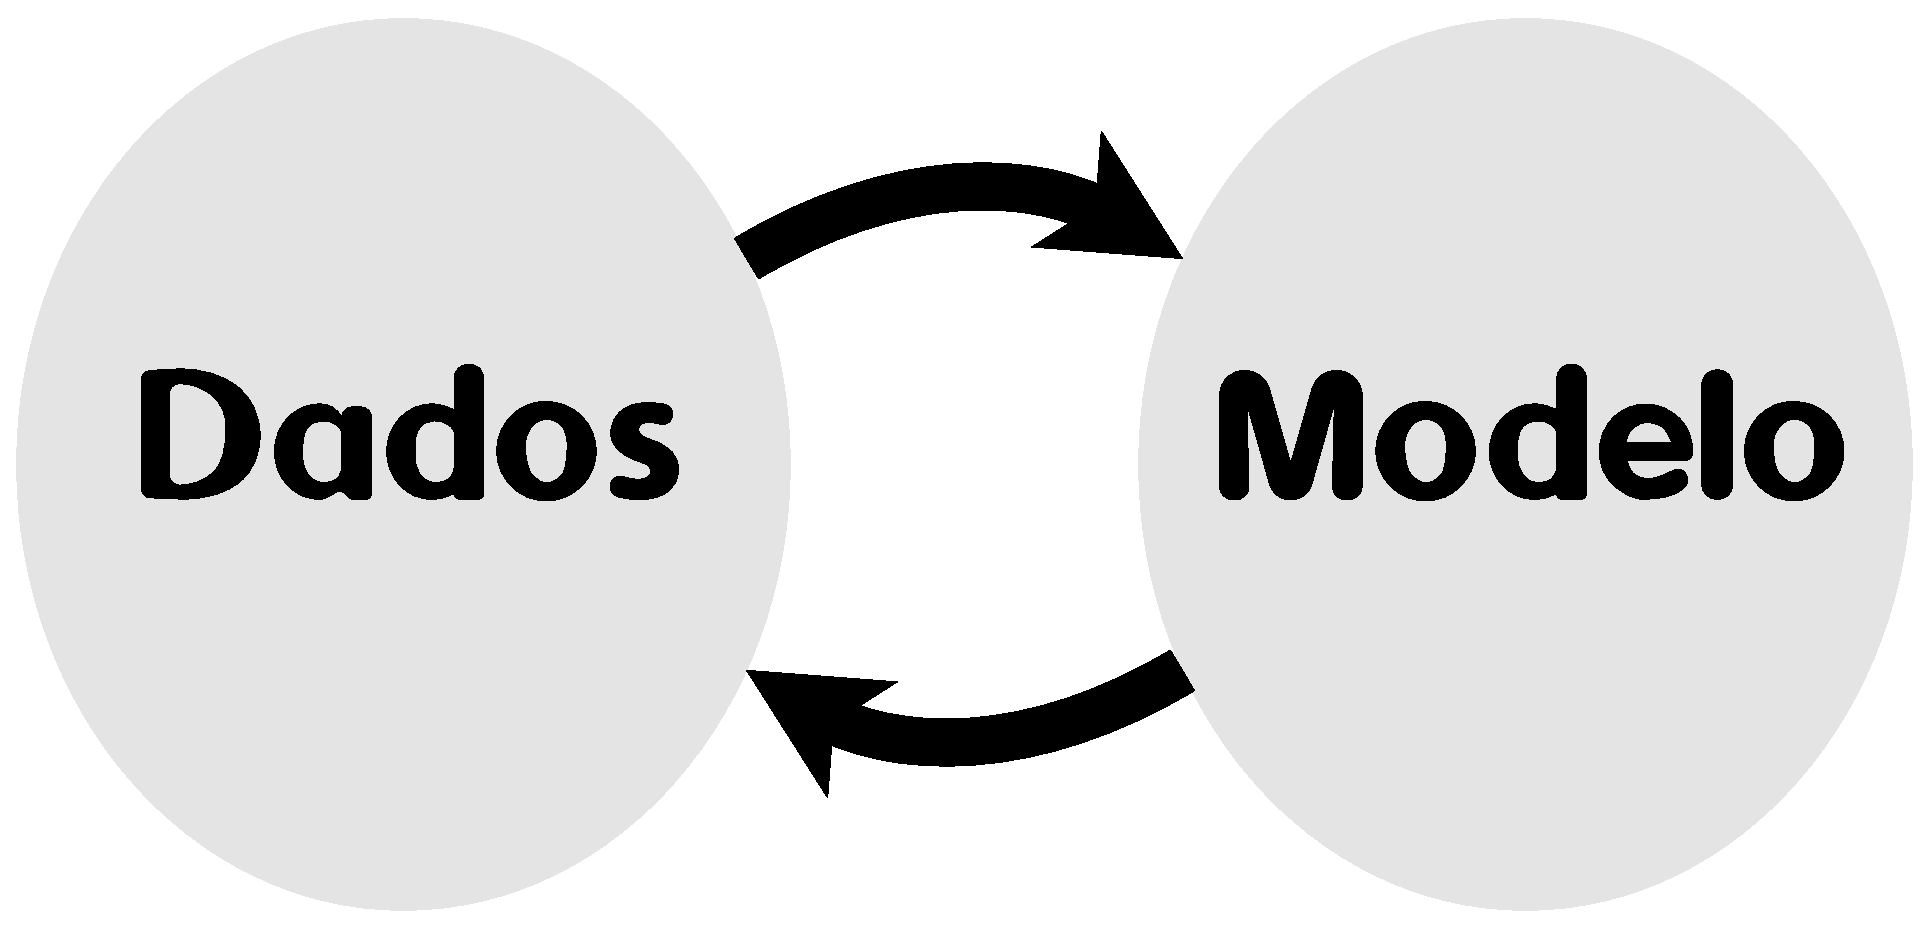
\includegraphics[width=0.3\textwidth]{principal}\\[1.0cm]
% pretitle
%{\fontsize{25}{30} \textsc{Algum pretitulo}}
% Title
\HRule{0.4cm} \\[0.4cm]
{ \fontsize{50}{60}   \bfseries \mytitle}\\[0.4cm]
\HRule{0.4cm} \\[0.7cm]
% SubTitle
{\fontsize{25}{30} \textsc{\mysubtitle}}\\[0.5cm]
\vfill
% Author 
\begin{minipage}{0.4\textwidth}
\begin{flushleft} \large
%\emph{Author:}\\
\myauthor %\textsc{Coppejans}
\end{flushleft}
\end{minipage}
% ID
\begin{minipage}{0.4\textwidth}
\begin{flushright} \large
\emph{Student number:} \\
sXXXXXXXX
\end{flushright}
\end{minipage}
% Bottom of the page
\vfill
{\large \imprimirdata}
\end{center}
\end{titlepage}
%% \end{comment}


%----------------------------------------------------------------------------------------
%	COPYRIGHT PAGE
%----------------------------------------------------------------------------------------
%\cleardoublepage

\newpage
\thispagestyle{empty}

\noindent Copyright \copyright\ \imprimiryear \myauthor\\ % Copyright notice

~\\

\noindent \textsc{Impresso no Brasil -- ISBN:\imprimirisbn}\\ % Publisher
\noindent \textsc{Publicado por \imprimireditora}\\ % Publisher
\noindent \textsc{Primeira impressão , \imprimirdata} % Printing/edition date

~\\

\textbf{Ficha catalográfica}
\begin{catalografica}%%
	\sffamily
	\vspace*{\fill}					% Posição vertical
	\begin{center}					% Minipage Centralizado
	\fbox{\begin{minipage}[c][5cm]{13.5cm}		% Largura
	\small
	\myauthor.
	%Sobrenome, Nome do autor
	
	\hspace{0.5cm} \mytitle: \mysubtitle   / \myauthor. --
	\imprimirlocal, \imprimiryear.
	
	\hspace{0.5cm} \pageref{LastPage} p. : il. (algumas color.) ; \imprimirsize.\\
	
	%\hspace{0.5cm} \imprimirorientadorRotulo~\imprimirorientador\\
	
	\hspace{0.5cm}
	\parbox[t]{\textwidth}{\imprimirtipotrabalho~--~\imprimireditora,~\imprimirdata.}\\

	\hspace{0.5cm}
	\parbox[t]{\textwidth}{ISBN:\imprimirisbn}\\


	
	\hspace{0.5cm}
		1. Métodos numéricos.
		2. Problemas inversos.
		3. Cáculo.
		I. Título 			
	\end{minipage}}
	\end{center}
\end{catalografica}%%

~\\

\noindent \textit{Garanta o ``download'' gratuito da versão digital do livro em \ImprimirLinkHomePageLivro}\\


\noindent Limite de responsabilidade e exceção de garantia: O autor ou autores tem feito
seu melhor esforço na preparação deste material.
Esta edição deve ser proporcionada sem nenhuma modificação. 
Se distribui gratuitamente com a esperança de que seja útil, 
porém sem nenhuma garantia expressa ou implícita em relação à exatidão ou completitude do conteúdo.


\vfill
\begin{wrapfigure}{l}{0.23\textwidth}

\includegraphics[height=32pt]{by-nc-nd.png}
\end{wrapfigure}
\noindent Esta obra está liberada com uma Licença 
Creative Commons Atribuição - NãoComercial - SemDerivações 4.0 Internacional.
Não é possível usar este arquivo excepto em conformidade com a Licença. 
Pode obter uma copia da Licença em:
\url{https://creativecommons.org/licenses/by-nc-nd/4.0/}\\ % License information


%----------------------------------------------------------------------------------------
%	DEDICATORIA
%----------------------------------------------------------------------------------------
\cleardoublepage

\null
\vfill
\thispagestyle{empty}



{\normalsize \it \hfill Amicum lege feliciter, vivas, gaudeas, floreas in Deo. \vspace*{4pt}

%\hfill understanding and assistance they have given me. \vspace*{4pt}

\hfill Fernando \vspace*{4pt}}

 

%----------------------------------------------------------------------------------------
%	Acknowledgements
%----------------------------------------------------------------------------------------
\cleardoublepage

\begin{center}
\Huge{\textbf{Agradecimentos}}
\end{center}

\null
\vfill
\thispagestyle{empty}

{\normalsize \it \hfill Dou muitas graças a Deus \vspace*{4pt}}


~\\

{\normalsize \it Dou muitas graças a XXXXX XXXXXXXXX por me 
ajudar a corrigir muitos dos erros na escrita do livro.
\vspace*{4pt}}

{\normalsize \it Dou muitas graças a XXXXX XXXXXXXXX por me 
ajudar a revisar a forma da escrita na linguagem matemática do livro.
\vspace*{4pt}}

\begin{comment}
{\normalsize \it Dou muitas graças a XXXXX XXXXXXXXX por me 
ajudar a resolver muitas duvidas sobre definições e uso de termos na XXXXXXX XXXXXXX.
\vspace*{4pt}}
\end{comment}

\begin{comment}
{\normalsize \it Dou muitas graças a XXXXX XXXXXXXXX pela 
suas sugestões e revisão  do capitulo XXXXX XXXXXXXXX.
\vspace*{4pt}}
\end{comment}


 

%----------------------------------------------------------------------------------------
%	PATROCINIO PAGE
%----------------------------------------------------------------------------------------
\cleardoublepage

\newpage
\thispagestyle{empty}


\begin{center}
\Huge{\textbf{Patrocínio}}
\end{center}

~\\

~\\



\begin{patrocinio}%%
	\sffamily
	\vspace*{\fill}					% Posição vertical
	\begin{center}					% Minipage Centralizado
	\fbox{\begin{minipage}[c][]{13.5cm}		% Largura

    ~\\

    \hspace{0.5cm}
    Para investir nesta pesquisa e colaborar com o desenvolvimento e crescimento deste projeto,
    você pode comprar um exemplar do livro. 
    Para ver uma lista com indicações sobre onde comprar:
    \begin{itemize}
    \item Uma versão impressa do livro, aceder a\\
    \ImprimirLinkCompraLivroImpresso 
    \item Uma versão digital do livro, aceder a\\
    \ImprimirLinkCompraLivroDigital \\ 
    \end{itemize}


    \hspace{0.5cm}
    Também pode colaborar com dinheiro em efetivo, desde 5 reais, 
    pelo seguinte método:
    \begin{itemize}
    \item \ImprimirLinkMetodoPagoA \\
    \end{itemize}


    \hspace{0.5cm} Para verificar a integridade do arquivo na versão digital deste livro,
    pode-se seguir as indicações publicadas no sitio oficial do projeto:
    \begin{itemize}
    \item \ImprimirLinkVerificarLivro \\
    \end{itemize}

    \hspace{0.5cm}
    Se já colaborou com a pesquisa, e se assim o deseja, 
    sintase livre de me mandar um e-mail a \ImprimirEmail, 
    sugerindo abordar um novo assunto ou aprofundar em outro.
    Se seu pedido está dentro das minhas capacidades 
    este será agregado sem falta na seguinte edição do livro.\\

    \begin{flushright}
    \myauthor ~\\ 
    \end{flushright}

	\end{minipage}}
	\end{center}
\end{patrocinio}%%



%----------------------------------------------------------------------------------------
%	My macros
%----------------------------------------------------------------------------------------
%% diagonal function
\newcommand{\funcdiag}{diag}


%% vectorization function
\newcommand{\funcvec}{vec}

%% transpose function
\newcommand{\functrans}{trans}
%% transpose operator
\newcommand{\transpose}{\mathrm{T}}

%% block matrix
\newcommand{\funcblockdiag}{blkdiag}
\newcommand{\funcblockhor }{blkhorz}
\newcommand{\funcblockver }{blkvert}



%----------------------------------------------------------------------------------------
%	TABLE OF CONTENTS
%----------------------------------------------------------------------------------------
\chapterimage{chapter_letras.pdf} % Table of contents heading image
\pagestyle{empty} % No headers
%\pagestyle{fancy} % Print headers again
\tableofcontents % Print the table of contents itself
\cleardoublepage % Forces the first chapter to start on an odd page so it's on the right
\pagestyle{fancy} % Print headers again

%----------------------------------------------------------------------------------------
%	PART
%----------------------------------------------------------------------------------------
\part{Teoria geral}
% CHAPTER  
%%%%%%%%%%%%%%%%%%%%%%%%%%%%%%%%%%%%%%%%%%%%%%%%%%%%%%%%%%%%%%%%%%%%%%%%%%%%%%%%
%%%%%%%%%%%%%%%%%%%%%%%%%%%%%%%%%%%%%%%%%%%%%%%%%%%%%%%%%%%%%%%%%%%%%%%%%%%%%%%%
%%%%%%%%%%%%%%%%%%%%%%%%%%%%%%%%%%%%%%%%%%%%%%%%%%%%%%%%%%%%%%%%%%%%%%%%%%%%%%%%
\section{Regressão}

\index{Regressão}

\begin{wrapfigure}{l}{0.5\textwidth}
     \centering
     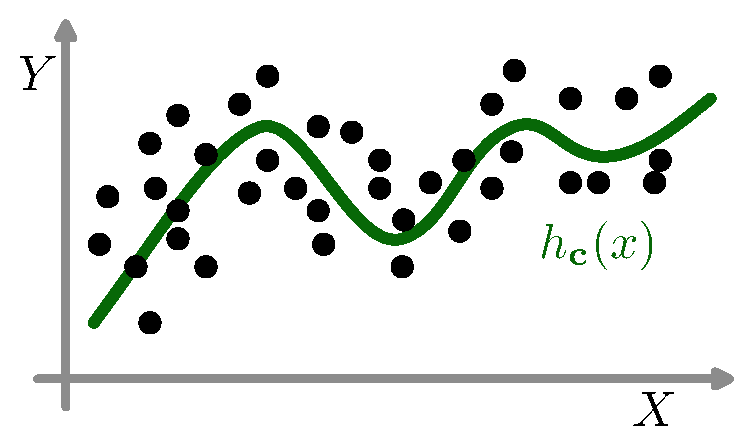
\includegraphics[width=0.45\textwidth]{chapters/notacao/regressao1.eps}
     \caption{Regressão de uma curva $h_{\VECTOR{c}}(x)$ com parâmetros $\VECTOR{c}$ num conjunto de dados. }
     \label{fig:regressao:1}
    \hspace{20pt}
\end{wrapfigure}
A regressão é o processo pelo qual uma curva ou superfície em múltiplas dimensões é 
ajustada num conjunto de dados, quando se sabe ou se aceita que existirá um erro no ajuste
devido à natureza ruidosa dos dados \cite[pp. 5]{chapra2016metodos}.

A ideia geral da regressão é achar uma curva de ajuste que represente melhor 
os dados, sem que a curva necessariamente coincida de forma exata com todos eles,
pelo que devemos definir algum critério de medida do erro de ajuste 
e procurar uma curva que minimize esse erro \cite[pp. 7]{chapra2016metodos}.

Assim, a regressão pode ser classificada mediante o tipo de curva de ajuste que é usado;
nesse sentido, podemos verificar na literatura:

\begin{itemize}
\item \textbf{Regressão linear}: 
Este caso ocorre quando usamos uma linha reta;
sendo esta uma função $h_{\VECTOR{c}}:\mathbb{R} \rightarrow \mathbb{R}$ de parâmetros $\VECTOR{c}$, 
utilizada para aproximar um conjunto de dados \cite[pp. 398, 402]{chapra2016metodos} \cite[pp. 25]{aster2013parameter}.
A regressão linear é um caso particular da regressão polinomial quando $M=1$.
\begin{example}~
\begin{itemize}
\item Curva de ajuste na regressão linear, 
\begin{equation}
h_{\VECTOR{c}}(x)=c_1+c_2 x.
\end{equation}
\item Na Seção \ref{sec:theo:reglogr1r1:1}, após uma linearização de uma relação não linear,
como na função logística, podemos ver exemplos de regressão linear.
\end{itemize}
\end{example}

\item \textbf{Regressão polinomial}: 
Indica que usamos um polinômio de grau $M$,
sendo esta uma função $h_{\VECTOR{c}}:\mathbb{R} \rightarrow \mathbb{R}$ com parâmetros $\VECTOR{c}$, 
utilizada para aproximar um conjunto de dados \cite[pp. 399, 415]{chapra2016metodos}.
\begin{example}~
\begin{itemize}
\item Curva de ajuste na regressão polinomial com grau $M=2$,
\begin{equation}
h_{\VECTOR{c}}(x)=c_1+c_2 x+c_3 x^2.
\end{equation}
\item Na Seção \ref{sec:theo:maphxr1r1}, podemos ver exemplos de regressão polinomial.
\item Na Seção \ref{sec:theo:reglogr1r1poly:1} após uma linearização de uma relação não linear,
como na função logística, podemos ver exemplos de regressão polinomial.
\end{itemize}
\end{example}

\item \textbf{Regressão não linear}: 
Neste caso, usamos um ajuste de dados
com uma função $h_{\VECTOR{c}}:\mathbb{R} \rightarrow \mathbb{R}$ com parâmetros $\VECTOR{c}$, 
que representa uma relação não linear entre o domínio e o contradomínio de $h_{\VECTOR{c}}$ 
\cite[pp. 424]{chapra2016metodos} \cite[pp. 217]{agarwal2014creators}.
\begin{example}~
\begin{itemize}
\item Um caso de curva de ajuste na regressão não linear, 
\begin{equation}
h_{\VECTOR{c}}(x)=c_1 e^{-c_2 x}.
\end{equation}
\item Na Seção \ref{sec:theo:maphcxr1r1}, podemos ver exemplos de regressão não linear.
\end{itemize}
\end{example}

\item \textbf{Regressão linear múltipla}:
Temos este caso quando ajustamos um hiperplano;
sendo esta uma função $h_{\VECTOR{c}}:\mathbb{R}^{N} \rightarrow \mathbb{R}$ com parâmetros $\VECTOR{c}$, 
utilizada para aproximar um conjunto de dados \cite[pp. 399, 418]{chapra2016metodos}.
A regressão linear é um caso particular da regressão linear múltipla quando $N=1$.
\begin{example}~
\begin{itemize}
\item Curva de ajuste na regressão linear múltipla com $N=2$, 
\begin{equation}
h_{\VECTOR{c}}(\VECTOR{x})=c_1+c_2 x_1+c_3 x_2.
\end{equation}
\item Na Seção \ref{sec:theo:reglogrnr1:1}, após uma linearização de uma relação não linear,
como na função logística, podemos ver exemplos de regressão linear múltipla.
\end{itemize}
\end{example}

\item \textbf{Regressão polinomial múltipla}:
Acontece quando ajustamos um polinômio multivariado de grau total $M$,
sendo esta uma função $h_{\VECTOR{c}}:\mathbb{R}^{N} \rightarrow \mathbb{R}$ com parâmetros $\VECTOR{c}$, 
utilizada para aproximar um conjunto de dados.
A regressão polinomial é um caso particular da regressão polinomial múltipla quando $N=1$.
\begin{example}~
\begin{itemize}
\item Um caso de curva de ajuste na regressão polinomial múltipla com 
$N=2$ e $h_{\VECTOR{c}}:\mathbb{R}^{2} \rightarrow \mathbb{R}$, 
\begin{equation}
h_{\VECTOR{c}}(\VECTOR{x})=c_1+c_2 x_1+c_3 x_2+c_4 x_1^2+c_5 x_2^2+c_6 x_1 x_2.
\end{equation}
\item Nas Seções \ref{sec:theo:maphxr2r1} e \ref{sec:theo:maphxr2r2},
 podemos ver exemplos de regressão polinomial múltipla.
\item Na Seção \ref{sec:theo:reglogrnr1poly:1}, após uma linearização de uma relação não linear,
como na função logística, podemos ver exemplos de regressão polinomial múltipla.
\end{itemize}
\end{example}

\item \textbf{Regressão não linear múltipla}: 
Estamos neste caso quado usamos no ajuste dos dados
uma função $h_{\VECTOR{c}}:\mathbb{R}^{N} \rightarrow \mathbb{R}$, 
que representa uma função não linear entre o domínio e o contradomínio de $h_{\VECTOR{c}}$.
A regressão não linear é um caso particular da regressão não linear múltipla quando $N=1$.
\begin{example}~
\begin{itemize}
\item Um caso de curva de ajuste na regressão não linear múltipla, 
\begin{equation}
h_{\VECTOR{c}}(\VECTOR{x})=c_1 e^{- c_2^2(x_1 -c_3)^2- c_4^2(x_2 -c_5)^2}.
\end{equation}
\item Na Seção \ref{sec:theo:maphcxrnr1}, podemos ver exemplos de regressão não linear múltipla.
\item Na Seção \ref{sec:theo:reglogrnr1nolinear:1}, após uma linearização de uma relação não linear,
como na função logística, podemos ver exemplos de regressão não linear múltipla.
\end{itemize}
\end{example}
\end{itemize}

\subsection{Linearização de curvas de ajuste não lineares}

Os problemas de \textbf{regressão não linear}
em alguns casos podem ser modificados para ter a forma de um 
problema de \textbf{regressão linear} (simples ou múltipla);
essa caraterística é interessante, pois geralmente
os problemas não lineares são resolvidos com métodos iterativos,
que podem ou não convergir na solução.
Em contrapartida, em problemas de regressão linear,
os métodos disponíveis nos brindam com uma resposta mediante um procedimento 
predeterminado, 
o que facilita o planejamento de um procedimento de solução e favorece o tempo de computo.

Assim, na continuação mostramos 
como problemas não lineares podem ser 
adaptados a um problema de regressão linear (simples):
\begin{example}
Usando 
$\hat{y}=ln(y)$,  
$\hat{x}=ln(x)$, 
$\hat{c}_1=ln(c_1)$, e
$\hat{c}_2=c_2$, obtemos %$\hat{y}=\hat{c}_1+\hat{c}_2 \hat{x}$.
\begin{equation}
y=c_1x^{c_2}
\quad \rightarrow \quad 
\hat{y}=\hat{c}_1+\hat{c}_2 \hat{x}.
\end{equation}
\vspace{-2pt}
\end{example}

\begin{example}%[Curva de ajuste $y=c_1 {c_2}^x$:]
Usando 
$\hat{y}=ln(y)$,  
$\hat{x}=x$, 
$\hat{c}_1=ln(c_1)$, e
$\hat{c}_2=ln(c_2)$, obtemos %$\hat{y}=\hat{c}_1+\hat{c}_2 \hat{x}$.
\begin{equation}
y=c_1 {c_2}^x
\quad \rightarrow \quad 
\hat{y}=\hat{c}_1+\hat{c}_2 \hat{x}.
\end{equation}
\vspace{-2pt}
\end{example}

\begin{example}%[Curva de ajuste $y=\left(c_1 + {c_2} x \right)^{-1}$:]
Usando 
$\hat{y}=\frac{1}{y}$,  
$\hat{x}=x$, 
$\hat{c}_1=c_1$, e 
$\hat{c}_2=c_2$, obtemos %$\hat{y}=\hat{c}_1+\hat{c}_2 \hat{x}$.
\begin{equation}
y=\left(c_1 + {c_2} x \right)^{-1}
\quad \rightarrow \quad 
\hat{y}=\hat{c}_1+\hat{c}_2 \hat{x}.
\end{equation}
\vspace{-2pt}
\end{example}

\begin{example}%[Curva de ajuste $y=c_1 x \left(c_2 + x\right)^{-1}$:] 
Usando 
$\hat{y}=\frac{1}{y}$,  
$\hat{x}=\frac{1}{x}$, 
$\hat{c}_1=\frac{1}{c_1}$, e 
$\hat{c}_2=\frac{c_2}{c_1}$, obtemos %$\hat{y}=\hat{c}_1+\hat{c}_2 \hat{x}$.
\begin{equation}
y=c_1 x \left(c_2 + x\right)^{-1}
\quad \rightarrow \quad 
\hat{y}=\hat{c}_1+\hat{c}_2 \hat{x}.
\end{equation}
\vspace{-2pt}
\end{example}

De forma similar ao caso de regressão linear simples,
curvas de ajuste não lineares podem ser adaptadas a um problema de regressão linear múltipla:
\begin{example}%[Curva de ajuste $y=c_1 +c_2 x + c_3 x^2 + c_4 x^3$:]
Usando 
$\hat{y}=y$,  
$\hat{x}_1=x$,
$\hat{x}_2=x^2$,
$\hat{x}_3=x^3$, 
$\hat{c}_1=c_1$, 
$\hat{c}_2=c_2$, 
$\hat{c}_3=c_3$, e 
$\hat{c}_4=c_4$, obtemos %$\hat{y}=\hat{c}_1+\hat{c}_2 \hat{x}_1+\hat{c}_2 \hat{x}_2+\hat{c}_3 \hat{x}_3$.
\begin{equation}
y=c_1 +c_2 x + c_3 x^2 + c_4 x^3
\quad \rightarrow \quad 
\hat{y}=\hat{c}_1+\hat{c}_2 \hat{x}_1+\hat{c}_2 \hat{x}_2+\hat{c}_3 \hat{x}_3.
\end{equation}
\vspace{-2pt}
\end{example}

\begin{example}%[Curva de ajuste $y=c_1 +c_2 \sqrt{x} + c_3 sin(x)$:]
Usando 
$\hat{y}=y$,  
$\hat{x}_1=\sqrt{x}$,
$\hat{x}_2=sin(x)$, 
$\hat{c}_1=c_1$, 
$\hat{c}_2=c_2$, e 
$\hat{c}_3=c_3$, obtemos %$\hat{y}=\hat{c}_1+\hat{c}_2 \hat{x}_1+\hat{c}_2 \hat{x}_2$.
\begin{equation}
y=c_1 +c_2 \sqrt{x} + c_3 sin(x)
\quad \rightarrow \quad 
\hat{y}=\hat{c}_1+\hat{c}_2 \hat{x}_1+\hat{c}_2 \hat{x}_2.
\end{equation}
\vspace{-2pt}
\end{example}

\newpage


%%%%%%%%%%%%%%%%%%%%%%%%%%%%%%%%%%%%%%%%%%%%%%%%%%%%%%%%%%%%%%%%%%%%%%%%%%%%%%%%%%%%%%%
%%%%%%%%%%%%%%%%%%%%%%%%%%%%%%%%%%%%%%%%%%%%%%%%%%%%%%%%%%%%%%%%%%%%%%%%%%%%%%%%%%%%%%%
%%%%%%%%%%%%%%%%%%%%%%%%%%%%%%%%%%%%%%%%%%%%%%%%%%%%%%%%%%%%%%%%%%%%%%%%%%%%%%%%%%%%%%%
\section{Regressão logística-fourier e SE com classificador $f_{\VECTOR{c}}(x):~\mathbb{R} \rightarrow \mathbb{R}$}
\label{sec:theo:reglogr1r1fourier:1}

\index{Regressão!Logística $f_{\VECTOR{c}}(x):~\mathbb{R} \rightarrow \mathbb{R}$}

\begin{theorem}[Classificação de dados em $\mathbb{R}$:]\label{theo:reglogr1r1fourier:1}
~\\
\noindent
\begin{minipage}{0.45\textwidth}
\centering
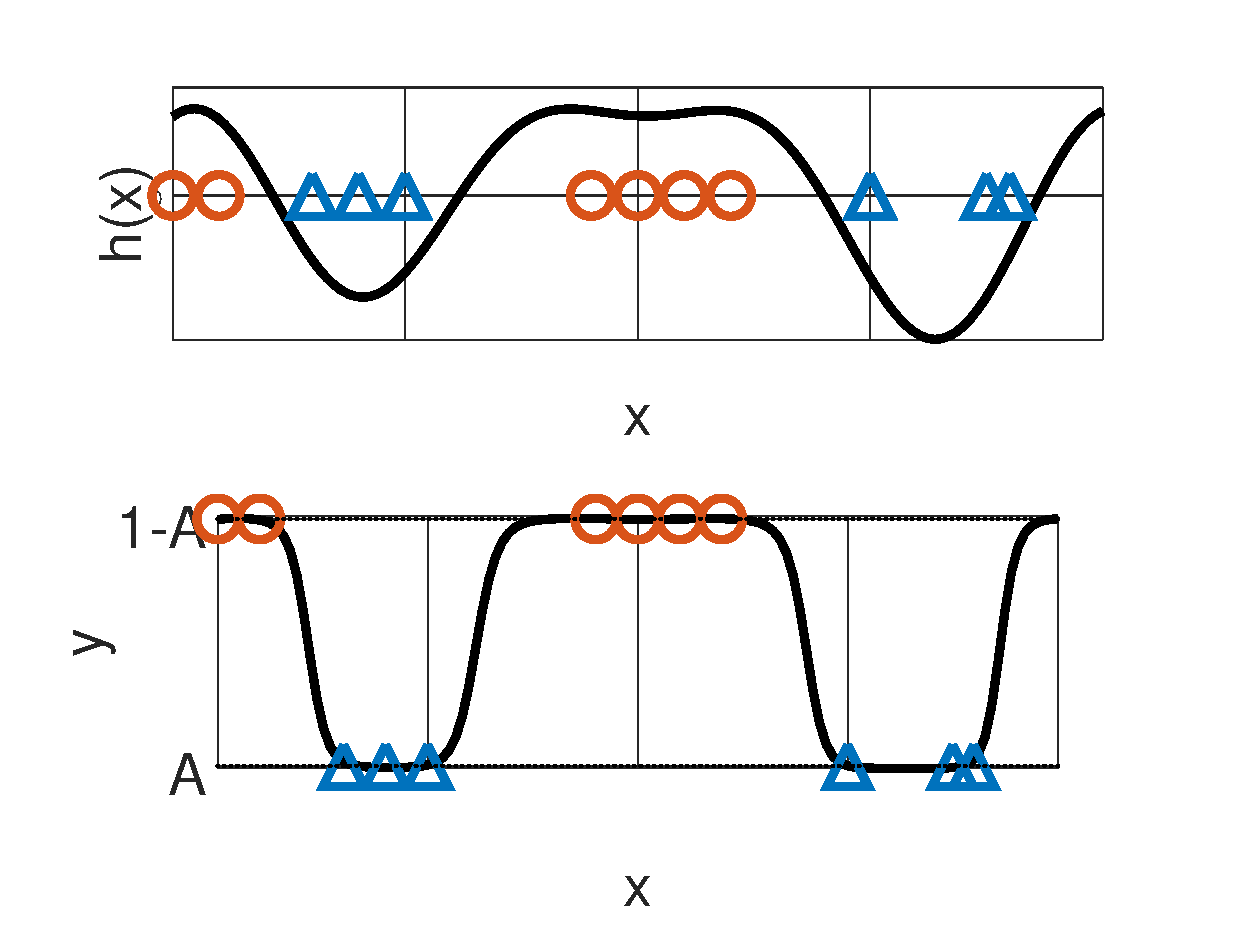
\includegraphics[width=0.95\linewidth]{chapters/classificacao/mfiles/reglogr1r1fourier/reglogr1r1fourier.eps} 
\end{minipage}
\begin{minipage}{0.55\textwidth}
Dados, um conjunto de $L$ dados $x_l \in \mathbb{R}, 1 \leq l \leq L$,
repartidos em dois grupos etiquetados com os símbolos $\bigtriangleup$ e $\bigcirc$, 
e separáveis por um hiperplano.
Se desejamos criar um classificador mediante 
a função  $f_{\VECTOR{c}}:\mathbb{R} \rightarrow \mathbb{R}$,
com domínio $x \in \mathbb{R}$, contradomínio $y \in \mathbb{R}$ e 
parâmetros agrupados no vetor $\VECTOR{c}=[c_1~ c_2~ ...~ c_{2 K+1}]^{\transpose}\in \mathbb{R}^{2 K+1}$,
como definido na Eq. (\ref{eq:reglogr1r1fourier:1}),
\begin{equation}\label{eq:reglogr1r1fourier:1}
y\equiv f_{\VECTOR{c}}(x)= \frac{1}{1+e^{-h_{\VECTOR{c}}(x) }},
\end{equation}
\end{minipage}
\begin{equation}
\quad h_{\VECTOR{c}}(x)=\frac{c_1}{2}+ \sum_{k=1}^{K} \left\{ 
c_{2k} sin\left(k \frac{2 \pi x}{L_x}\right) + 
c_{2k+1} cos\left(k \frac{2 \pi x}{L_x}\right)
\right\},
\end{equation}
ou seu equivalente: $logit(y)=h_{\VECTOR{c}}(x)$, onde\footnote{Tem 
que ser maior para evitar erros de $f_{\VECTOR{c}}(x)$ nos extremos. 
Ex.: $L_x =1.1 || max(x_i)-min(x_i)||$.}
 $L_x > || max(x_i)-min(x_i)||$.

Podemos atribuir a cada valor $x_l$ uma etiqueta $y_l\in \{A,1-A\}$, 
onde $0<A\ll 0.5$ é escolhido por nós,
e afirmar que o vetor $\VECTOR{c}= \VECTOR{\hat{c}}$,
que minimiza o erro quadrático $e(\VECTOR{c})$,
\begin{equation}\label{eq:reglogr1r1fourier:1e}
e(\VECTOR{c}) =  \sum_{l=1}^{L} w_l||h_{\VECTOR{c}}(x_l) -logit(y_l)||^2,
\end{equation}
ponderado usando os pesos $w_l \in \mathbb{R}_+$, 
pode ser achado\footnote{A demostração pode ser vista na Prova \ref{proof:theo:reglogr1r1fourier}.}  
com
\begin{equation}\label{eq:reglogr1r1fourier:2}
\VECTOR{\hat{c}} =  \left[ \MATRIX{A}^{\transpose} \MATRIX{W}\MATRIX{A}\right]^{-1} \MATRIX{A}^{\transpose} \MATRIX{W}\VECTOR{z},
\quad
\MATRIX{A}=
\begin{bmatrix}
\VECTOR{a}_{K}(x_1) \\
\VECTOR{a}_{K}(x_2) \\
\vdots \\
\VECTOR{a}_{K}(x_l) \\
\vdots \\
\VECTOR{a}_{K}(x_L) \\
\end{bmatrix},
\quad
\MATRIX{W}=\funcdiag \left(
\begin{bmatrix}
w_1  \\
w_2  \\
\vdots  \\
w_l  \\
\vdots \\
w_L \\
\end{bmatrix}
\right),
\quad
\VECTOR{z}=
\begin{bmatrix}
logit(y_1)  \\
logit(y_2)  \\
\vdots  \\
logit(y_l)  \\
\vdots \\
logit(y_L) \\
\end{bmatrix},
\end{equation}
\begin{equation}
\VECTOR{a}_{K}(x)=
\begin{bmatrix}
\frac{1}{2} & 
sin\left( \frac{2 \pi x}{L_x}\right) & 
cos\left( \frac{2 \pi x}{L_x}\right) &
%sin\left(2 \frac{2 \pi x}{L_x}\right) & 
%cos\left(2 \frac{2 \pi x}{L_x}\right) &
\dots &
sin\left(K \frac{2 \pi x}{L_x}\right) & 
cos\left(K \frac{2 \pi x}{L_x}\right)
\end{bmatrix}.
\end{equation}
\end{theorem}
\begin{tcbattention}
\begin{itemize}
\item Dado que a função de classificação $f_{\VECTOR{c}}(x)$ vai entre $0$ e $1$,
podemos reinterpretar este valor como se fosse uma probabilidade;
neste caso, $f_{\VECTOR{c}}(x_l)$ representa, $P(y_l=\bigcirc|x_l)$, 
a probabilidade de que $y_l=\bigcirc$ dado que tivemos como entrada o valor $x_l$.
%\item O limiar da classificação de $f_{\VECTOR{c}}(x)$ 
%está no hiperplano $h_{\VECTOR{c}}(x)=0$,
%provocando neste ponto um $f_{\VECTOR{c}}(x)=0.5$.
\item $L_x$ indica o periodo de repetição do classificador,
por este motivo o classificador é interessante quando o domínio dos dados ($x_l$) está restrito.
\end{itemize}
\end{tcbattention}


\newpage


%%%%%%%%%%%%%%%%%%%%%%%%%%%%%%%%%%%%%%%%%%%%%%%%%%%%%%%%%%%%%%%%%%%%%%%%%%%%%%%%%%%%%%%
%%%%%%%%%%%%%%%%%%%%%%%%%%%%%%%%%%%%%%%%%%%%%%%%%%%%%%%%%%%%%%%%%%%%%%%%%%%%%%%%%%%%%%%
%%%%%%%%%%%%%%%%%%%%%%%%%%%%%%%%%%%%%%%%%%%%%%%%%%%%%%%%%%%%%%%%%%%%%%%%%%%%%%%%%%%%%%%
\section{\textcolor{red}{Regressão logística-fourier e SE com classificador $f_{\VECTOR{c}}(\VECTOR{x}):~\mathbb{R}^{N} \rightarrow \mathbb{R}$}}
\label{sec:theo:reglogrnr1fourier:1}

\index{Regressão!Logística $f_{\VECTOR{c}}(\VECTOR{x}):~\mathbb{R}^{N} \rightarrow \mathbb{R}$}

\begin{theorem}[Classificação de dados em $\mathbb{R}$:]\label{theo:reglogrnr1fourier:1}
~\\
\noindent
\begin{minipage}{0.45\textwidth}
\centering
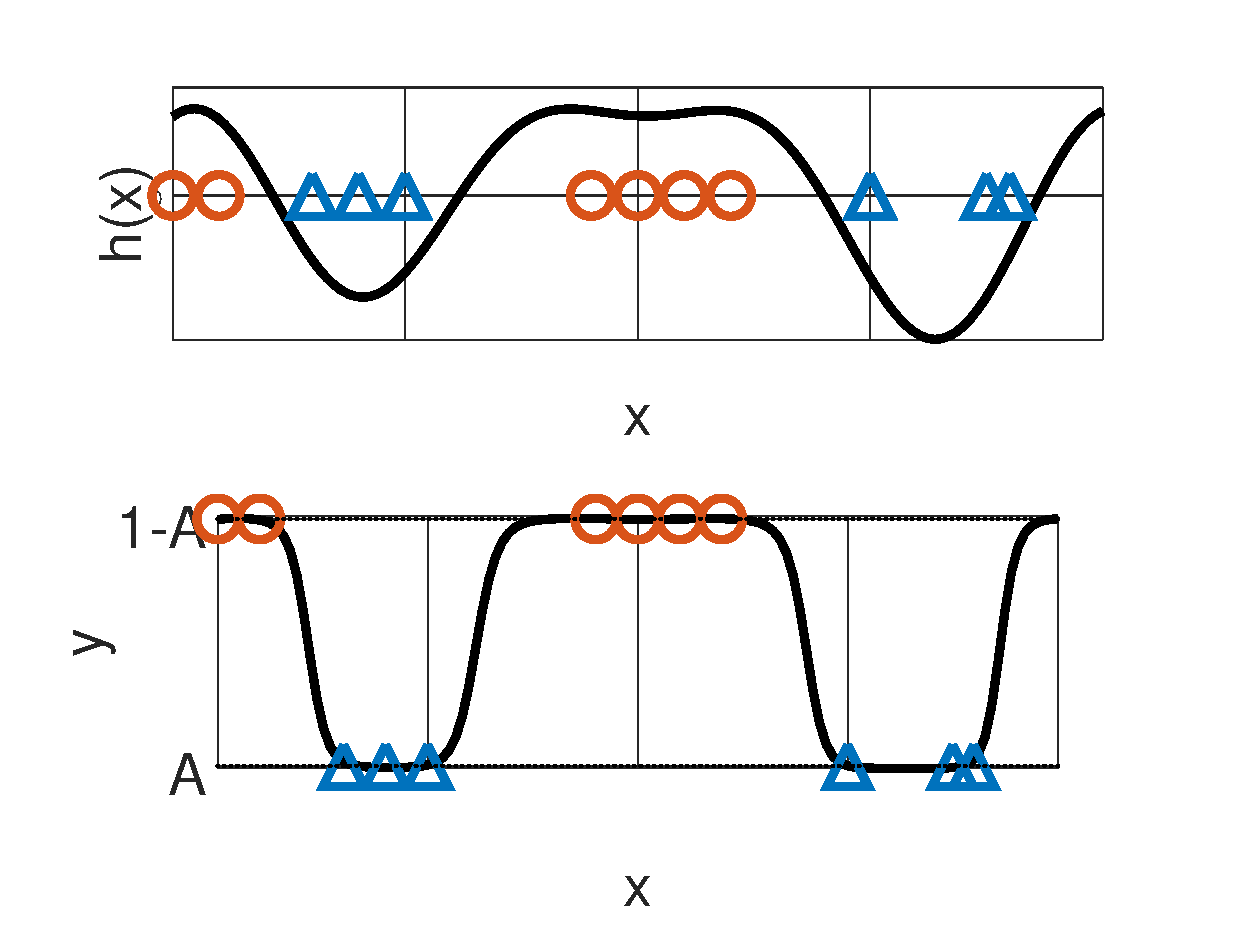
\includegraphics[width=0.95\linewidth]{chapters/classificacao/mfiles/reglogrnr1fourier/reglogrnr1fourier.eps} 
\end{minipage}
\begin{minipage}{0.55\textwidth}
Dados, um conjunto de $L$ pontos $\VECTOR{x}_l \in \mathbb{R}, 1 \leq l \leq L$,
repartidos em dois grupos etiquetados com os símbolos $\bigtriangleup$ e $\bigcirc$, 
e separáveis por um hiperplano.
Se desejamos criar um classificador mediante 
a função  $f_{\VECTOR{c}}:\mathbb{R}^{N} \rightarrow \mathbb{R}$,
com domínio $\VECTOR{x} \in \mathbb{R}^{N}$, contradomínio $y \in \mathbb{R}$ e 
parâmetros agrupados no vetor $\VECTOR{c}=[c_1~ c_2~ ...~ c_{2M}]^{\transpose}\in \mathbb{R}^{2 M}$, 
$M={(2 K+1)}^N$,
como definido na Eq. (\ref{eq:reglogrnr1fourier:1}),
\begin{equation}\label{eq:reglogrnr1fourier:1}
y\equiv f_{\VECTOR{c}}(\VECTOR{x})= \frac{1}{1+e^{-h_{\VECTOR{c}}(\VECTOR{x}) }},
\end{equation}
\end{minipage}
\begin{equation}
 h_{\VECTOR{c}}(\VECTOR{x}) = 
\sum_{\VECTOR{k}=\VECTOR{k}_1}^{\VECTOR{k}_M}
a_{\VECTOR{k}} cos\left(\VECTOR{k}^{\transpose}\MATRIX{W}_{L}\VECTOR{x}\right)+
b_{\VECTOR{k}} sin\left(\VECTOR{k}^{\transpose}\MATRIX{W}_{L}\VECTOR{x}\right),
\end{equation}


ou seu equivalente: $logit(y)=h_{\VECTOR{c}}(\VECTOR{x})$, onde a matriz
$\MATRIX{W}_{L}=\funcdiag\left(\left[\frac{2 \pi}{L_1},~\frac{2 \pi}{L_2},~\dots,~\frac{2 \pi}{L_N}\right]^{\transpose}\right)$
e\footnote{Tem 
que ser maior para evitar erros de $f_{\VECTOR{c}}(\VECTOR{x})$ nos extremos. 
Ex.: $L_n =1.1 || max(x_n)-min(x_n)||$.}
 $L_n > || max(x_n)-min(x_n)||$.

Podemos atribuir a cada valor $\VECTOR{x}_l$ uma etiqueta $y_l\in \{A,1-A\}$, 
onde $0<A\ll 0.5$ é escolhido por nós,
e afirmar que o vetor $\VECTOR{c}= \VECTOR{\hat{c}}$,
que minimiza o erro quadrático $e(\VECTOR{c})$,
\begin{equation}\label{eq:reglogrnr1fourier:1e}
e(\VECTOR{c}) =  \sum_{l=1}^{L} q_l||h_{\VECTOR{c}}(\VECTOR{x}_l) -logit(y_l)||^2,
\end{equation}
ponderado usando os pesos $q_l \in \mathbb{R}_+$, 
pode ser achado\footnote{A demostração pode ser vista na Prova \ref{proof:theo:reglogrnr1fourier}.}  
com
\begin{equation}\label{eq:reglogrnr1fourier:2}
\VECTOR{\hat{c}} =  \left[ \MATRIX{A}^{\transpose} \MATRIX{Q}\MATRIX{A}\right]^{-1} \MATRIX{A}^{\transpose} \MATRIX{Q}\VECTOR{z},
\quad
\MATRIX{A}=
\begin{bmatrix}
\VECTOR{a}_{K}(\VECTOR{x}_1) & \VECTOR{b}_{K}(\VECTOR{x}_1) \\
\VECTOR{a}_{K}(\VECTOR{x}_2) & \VECTOR{b}_{K}(\VECTOR{x}_2) \\
\vdots \\
\VECTOR{a}_{K}(\VECTOR{x}_l) & \VECTOR{b}_{K}(\VECTOR{x}_l) \\
\vdots \\
\VECTOR{a}_{K}(\VECTOR{x}_L) & \VECTOR{b}_{K}(\VECTOR{x}_L) \\
\end{bmatrix},
\quad
\MATRIX{Q}=\funcdiag \left(
\begin{bmatrix}
q_1  \\
q_2  \\
%\vdots  \\
%q_l  \\
\vdots \\
q_L \\
\end{bmatrix}
\right),
\quad
\VECTOR{z}=
\begin{bmatrix}
logit(y_1)  \\
logit(y_2)  \\
%\vdots  \\
%logit(y_l)  \\
\vdots \\
logit(y_L) \\
\end{bmatrix},
\end{equation}
\begin{equation}
\VECTOR{a}_{K}(\VECTOR{x})=
\begin{bmatrix}
cos\left(\VECTOR{k}_{1}^{\transpose}\MATRIX{W}_{L}\VECTOR{x}\right) &
cos\left(\VECTOR{k}_{2}^{\transpose}\MATRIX{W}_{L}\VECTOR{x}\right) &
\dots  &
cos\left(\VECTOR{k}_{M}^{\transpose}\MATRIX{W}_{L}\VECTOR{x}\right)
\end{bmatrix},
\end{equation}
\begin{equation}
\VECTOR{b}_{K}(\VECTOR{x})=
\begin{bmatrix}
sin\left(\VECTOR{k}_{1}^{\transpose}\MATRIX{W}_{L}\VECTOR{x}\right) &
sin\left(\VECTOR{k}_{2}^{\transpose}\MATRIX{W}_{L}\VECTOR{x}\right) &
\dots  &
sin\left(\VECTOR{k}_{M}^{\transpose}\MATRIX{W}_{L}\VECTOR{x}\right)
\end{bmatrix}.
\end{equation}
\end{theorem}
\begin{tcbattention}
\begin{itemize}
\item Dado que a função de classificação $f_{\VECTOR{c}}(\VECTOR{x})$ vai entre $0$ e $1$,
podemos reinterpretar este valor como se fosse uma probabilidade;
neste caso, $f_{\VECTOR{c}}(\VECTOR{x})$ representa a probabilidade de que um valor $\VECTOR{x}$
pertença ao grupo $\bigcirc$.
\item O limiar da classificação de $f_{\VECTOR{c}}(\VECTOR{x})$ 
está no hiperplano $h_{\VECTOR{c}}(\VECTOR{x})=0$,
provocando neste ponto um $f_{\VECTOR{c}}(\VECTOR{x})=0.5$.
\item $L_x$ indica o periodo de repetição do classificador,
por este motivo o classificador é interessante quando o domínio dos dados ($\VECTOR{x}_l$) está restrito.
\end{itemize}
\end{tcbattention}


\begin{proof}[Relativa ao Teorema \ref{sec:theo:reglogrnr1fourier:1}:]

\textcolor{red}{Fingerprint a detectar surcos}\\

\begin{equation}
 h_{\VECTOR{c}}(\VECTOR{x}) = 
\sum_{\VECTOR{k}=[-K,~ ...,-K]}^{[K,~ ...,~K]}
c_{\VECTOR{k}}  e^{\mathbf{i}\VECTOR{k}^{\transpose}\MATRIX{W}_{L}\VECTOR{x}},
\quad 
\MATRIX{W}_{L}=\funcdiag\left(\left[\frac{2 \pi}{L_1},~\frac{2 \pi}{L_2},~\dots,~\frac{2 \pi}{L_N}\right]^{\transpose}\right)
\end{equation}
\begin{equation}
 h_{\VECTOR{c}}(\VECTOR{x}) = 
\sum_{\VECTOR{k}=[-K,~ ...,-K]}^{[K,~ ...,~K]}
Re\left\{c_{\VECTOR{k}}\right\}cos\left(\VECTOR{k}^{\transpose}\MATRIX{W}_{L}\VECTOR{x}\right)
-Im\left\{c_{\VECTOR{k}}\right\}sin\left(\VECTOR{k}^{\transpose}\MATRIX{W}_{L}\VECTOR{x}\right),
\end{equation}
\begin{equation}
 h_{\VECTOR{c}}(\VECTOR{x}) = 
\sum_{\VECTOR{k}=[-K,~ ...,-K]}^{[K,~ ...,~K]}
a_{\VECTOR{k}} cos\left(\VECTOR{k}^{\transpose}\MATRIX{W}_{L}\VECTOR{x}\right)+
b_{\VECTOR{k}} sin\left(\VECTOR{k}^{\transpose}\MATRIX{W}_{L}\VECTOR{x}\right),
\end{equation}

\end{proof}



%----------------------------------------------------------------------------------------
%----------------------------------------------------------------------------------------
%----------------------------------------------------------------------------------------
%	Apendice
%----------------------------------------------------------------------------------------
%\part{Apendice}


%----------------------------------------------------------------------------------------
%	BIBLIOGRAPHY
%----------------------------------------------------------------------------------------
%----------------------------------------------------------------------------------------
%----------------------------------------------------------------------------------------
%----------------------------------------------------------------------------------------
%	PART
%----------------------------------------------------------------------------------------
\part{Referências}


\chapterimage{chapter_livro.pdf}

\chapter*{Bibliografia}
\addcontentsline{toc}{chapter}{\textcolor{colorsystemdefault}{Bibliografia}} %% Sale en la pagina part

\newrefcontext[sorting=nty]

\section*{Livros}
\addcontentsline{toc}{section}{Livros} %% Sale en la pagina part
\printbibliography[heading=bibempty,type=book]

\section*{Artigos}
\addcontentsline{toc}{section}{Artigos} %% Sale en la pagina part
\printbibliography[heading=bibempty,type=article]

\section*{Outras fontes}
\addcontentsline{toc}{section}{Outras fontes} %% Sale en la pagina part
\printbibliography[heading=bibempty, nottype=article, nottype=book]


%----------------------------------------------------------------------------------------
%	INDEX
%----------------------------------------------------------------------------------------

\chapterimage{chapter_letras.pdf}

\cleardoublepage
\phantomsection
\setlength{\columnsep}{0.75cm}
\addcontentsline{toc}{chapter}{\textcolor{colorsystemdefault}{Índice}} %% Sale en la pagina part
\printindex

%----------------------------------------------------------------------------------------

%----------------------------------------------------------------------------------------
%	COLOFÃO
%----------------------------------------------------------------------------------------
\cleardoublepage

\null
\vfill
\newpage

\null
\vfill
\thispagestyle{empty}


{\normalsize \it Este livro foi produzido por \myauthor, editado e diagramado usando \LaTeX,
usando um tipo de fonte \showfont,
para ser impresso num papel tamanho \ImprimirTamanhoPapel,  \imprimirdata.
\vspace*{4pt}}








\end{document}
